\documentclass[11pt]{book}
\usepackage{graphicx}
\DeclareGraphicsRule{.tiff}{png}{.png}{`convert #1 `dirname #1`/`basename #1 .tiff`.png}

\usepackage{amsmath,amssymb}
\usepackage{times}
\usepackage{epstopdf}
\usepackage[ligature,reserved]{semantic}
\usepackage[center,tight]{subfigure}

\textwidth = 6.5 in
\textheight = 9 in
\oddsidemargin = 0.0 in
\evensidemargin = 0.0 in
\topmargin = 0.0 in
%\headheight = 0.0 in
%\headsep = 0.0 in
\parskip = 3pt
\parindent = 0.0in

%no indent on footnotes
\makeatletter
\renewcommand{\@makefntext}[1]{\setlength{\parindent}{0pt}%
\begin{list}{}{\setlength{\labelwidth}{1em}%
  \setlength{\leftmargin}{\labelwidth}%
  \setlength{\labelsep}{3pt}\setlength{\itemsep}{0pt}%
  \setlength{\parsep}{0pt}\setlength{\topsep}{0pt}%
  \footnotesize}\item[\hfill\@makefnmark]#1%
\end{list}}
\makeatother

%\newtheorem{theorem}{Theorem}
%\newtheorem{corollary}[theorem]{Corollary}
%\newtheorem{definition}{Definition}

\title{\huge Natural Deduction Proof and Disproof in Jape}
\author{Richard Bornat (richard@bornat.me.uk)}

\mathlig{->}{\rightarrow}
\mathlig{|-}{\vdash}
\mathlig{|=}{\vDash}
\mathlig{|*}{\exists}
\mathlig{|}{\lor}
\mathlig{!}{\neg}
\mathlig{@*}{\forall}
\mathlig{@}{\land}

\reservestyle{\word}{\operatorname}
\word{actual}

\reservestyle{\var}{\mathit}
\var{j1,j2}

\newcommand{\eqnref}[1]{(\ref{eqn:#1})}
\newcommand{\figref}[1]{figure \ref{fig:#1}}
\newcommand{\Figref}[1]{Figure \ref{fig:#1}}
\newcommand{\secref}[1]{section \ref{sec:#1}}
\newcommand{\Secref}[1]{Section \ref{sec:#1}}
\newcommand{\chapref}[1]{chapter \ref{chap:#1}}
\newcommand{\Chapref}[1]{Chapter \ref{chap:#1}}

\begin{document}
\maketitle

\chapter*{Preface}

This manual is a how-to for Jape. Earlier versions contained a good deal of logic teaching. That's been dropped, since now there's a book (Logic for Programmers, OUP) which says it all a good deal better. You will learn about logic by playing with Jape, so I suppose there's still teaching in there.

This document was written on a Mac, and the illustrations are all taken from the MacOS X version of Jape. All Japes, on Linux, Solaris, Windows, MacOS X or whereever, run exactly the same code but the interfaces can look slightly different. I haven't produced different versions of the manual because I think --- rather, I hope --- that those differences in fonts, in window controls, in the placing of menus and so on, don't really matter. If I'm wrong then I hope somebody will tell me.

\section*{Jape or NDJape?}

This manual is really about how Jape, which is capable of working with many different logics, has been made to deal with Natural Deduction as described in my book. Instead of talking about what `Jape' does when dealing with $->$ formulae, I should really talk about what `Jape loaded with the I2L encoding' does. But that's such a mouthful that I just talk as if there is only one Jape, and all it does is Natural Deduction.

If you're interested there's a manual on the website (http://www.jape.org.uk) which tells you how to roll your own logic encodings. Best of luck.

\section{Differences from the book}
\begin{itemize}
\item Jape writes its premises on a single line, separated by commas, instead of using a separate line for each premise;
\item Jape writes quantifications as $@*x.P(x)$ and $|*y.Q(y)$ --- with a dot between bound variable and predicate --- instead of $@*x(P(x))$ and $|*y(Q(y))$
\end{itemize}
So far as I know, these are the only significant differences.

\section*{Any comments?}

If Jape doesn't work for you, it isn't working, and if it isn't working I'd like to hear about it. 

Please send any comments, thoughts, complaints or whatever to bugs@jape.org.uk. I'll do my best to reply quickly and if your message is of general interest I'll put it up on the website (though of course, because of spambots, I'll hide your email address). 

\section*{Acknowledgements}

I designed and built Jape between 1991 and 2002 whilst I was at Queen Mary College, University of London. For the first four years or so I worked closely with Bernard Sufrin of the Computer Laboratory, Oxford University. Bernard's design insights were crucial and without him Jape wouldn't exist or be half as good as it is. His program architecture, which he worked out in the first few months of our collaboration, is still in place even though Jape has been rebuilt more than once. He still works with me on producing the Windows, Linux and Solaris distributions.

For the rest of it I've been strongly influenced by colleagues at Queen Mary, many of whom have made seminal suggestions which have improved Jape. In alphabetical order I single out Jules Bean, John Bell, Peter Burton, Keith Clarke, Adam Eppendahl, David Pym, Graem Ringwood, Mike Samuels, Paul Taylor and Graham White. 

Jape began as an experiment towards the end of an EPSRC research project on the use of symbolic calculators to teach formal reasoning, joint with Steve Reeves and Doug Goldson at Queen Mary, and Tim O'Shea and Pat Fung at the Open University. A later project, with Pat Fung and James Aczel from the OU, looked at students using Jape; James's insightful summary of their difficulties led to a redesign of the treatment of natural deduction, and directly to this version of the program.

Jape's proof engine was originally written in SML and compiled by SMLNJ, with interfaces for different operating systems written in C, tcl/tk, Python and I can't remember what else. In 2002 I ported the engine to OCaml and wrote a system-independent interface module in Java. I'm grateful to the implementers of all those languages, especially for their decision to provide their software for free. Jape is free too, at http:www.jape.org.uk. 

In what follows the mistakes are all my own.

\chapter{Basics}

\begin{figure}
\centering
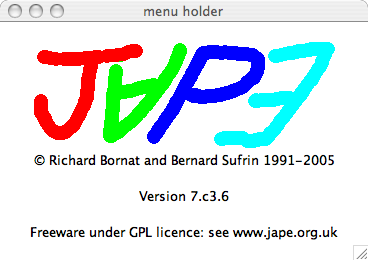
\includegraphics[scale=0.5]{pics/splashscreen.png}
\caption{The Jape splash screen}
\label{fig:splashscreen}
\end{figure}
\begin{figure}
\centering
\parbox[b]{165pt}{\centering
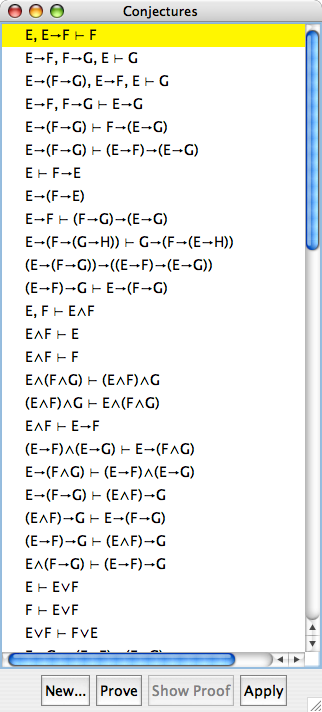
\includegraphics[scale=0.5]{pics/conjecturespanel.png}
\caption{The Conjectures panel}
\label{fig:conjecturespanel}}
\qquad
\parbox[b]{230pt}{\centering
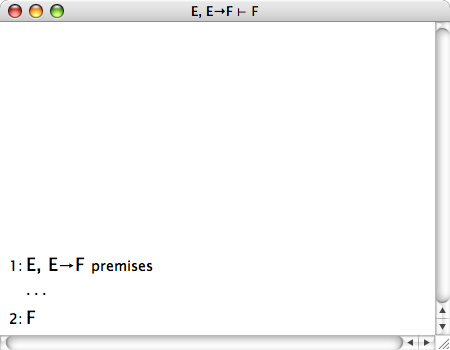
\includegraphics[scale=0.5]{pics/firstproofwindow.png}
\caption{A proof window}
\label{fig:firstproofwindow}}
\end{figure}

\section{Getting started}

If you don't already have Jape, download it from http://www.jape.org.uk. Install it, following the instructions carefully.

You should have a directory containing Jape, another program called jape\_engine, and a subdirectory called examples. Double-click Jape, and you will see a window like \figref{splashscreen}.\footnote{You may see minor differences. The illustrations in this manual are taken from MacOS X. On Windows and Linux you will see a menu bar in the window and the window title will be Jape. But those differences don't matter much, so I won't refer to them again.}

Using the Open New Theory command in  the File menu, open examples/natural\_deduction/I2L.jt. You should see several windows containing logical conjectures (claims to be proved), called \emph{panels} in Jape. The Conjectures panel should look something like \figref{conjecturespanel} (you will probably have to resize the window to make it look like this). Double-click any line to begin, or select a line and press the Prove button at the bottom of the panel. You will see a \emph{proof window} like \figref{firstproofwindow}, and off you go!

\begin{figure}
\centering
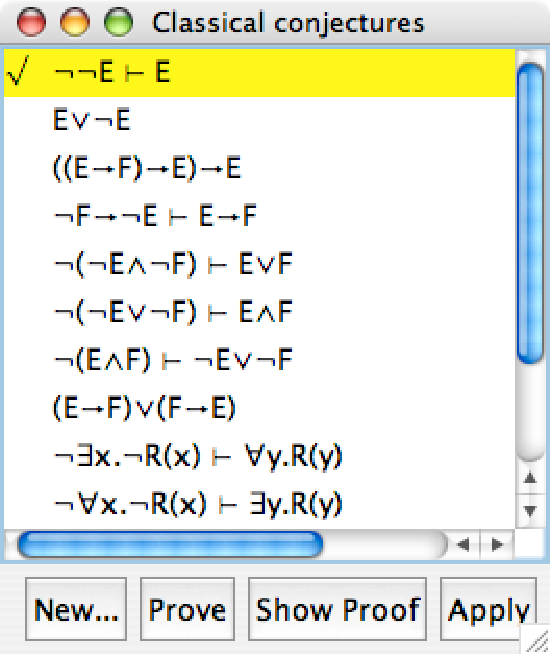
\includegraphics[scale=0.5]{pics/provedconjecture}
\caption{A conjecture panel with a proved conjecture}
\label{fig:provedconjecture}
\end{figure}

\section{Finishing a proof}

When you have made a proof of a conjecture --- no more lines of dots in the proof window --- you can save it: pull down the Edit menu and select Done. The proof window closes, and Jape records the fact that the conjecture is proved, marking its entry in the conjectures panel with a tick in the margin, as illustrated in \figref{provedconjecture}.

Proof of a conjecture makes it a theorem. You can use theorems in your proofs as if they were additional Natural Deduction rules by using the Conjectures panel's Apply button, and you can review 
their proofs using the Show Proof button.

\section{Saving and restoring your work}

Jape offers to record your proofs --- saved and unsaved --- when you quit or when you choose ``Save Proofs'' or ``Save Proofs As ...'' from the File menu. It will reload saved proofs using ``Open ...'', also from the File menu. 

\section{Making Jape work for you}

\subsection{Only reflect}

Jape is designed to be easy to use, which means that the mouse and menu and window stuff don't get in the way of the logic. It's so easy to use that you can have great fun clicking away, `solving' lots of problems without always knowing exactly what you're doing. That's ok, because you can learn while you're having fun, and you can do things for yourself without asking for help. But it's obviously not the whole story.

Because Jape is easy to use it brings you quickly to a point where you can ask interesting and important questions. The kind of question you are supposed to ask is ``is the logic really supposed to work like \emph{that}?'' If there are experts around you can ask them, but if you are on your own you can still ask yourself. That isn't a daft thing to do: educationalists call it \emph{reflection}, and it's one of the best ways to learn.

Some logical proofs are hard to believe at first. Some single logical steps are pretty surprising. I hope that you will always read through finished Jape proofs to see if you can believe them. If there is a surprise, ask yourself: where does the surprise come from? By undoing and redoing steps you can watch the surprise emerge and explain to yourself why it's necessary.

Jape's a kind of machine, and that has disadvantages as well as advantages. The big advantage is that a machine can do formal calculation --- proof and disproof --- perfectly, without mistake. The big disadvantage is that it can't understand anything about what it's doing. Jape doesn't know the difference between a nice proof and a nasty one. Sometimes reflection will show you that there is a shorter or prettier proof than the one you have made. You can always undo your work and try again!

\subsection{Be brave}

We read proofs top-to-bottom most of the time. Novices, quite reasonably, imagine that proofs are constructed top-to-bottom too: start at line 1 and work forwards. Well, sometimes it is done that way, but at least as often it's done the other way round, bottom-to-top, starting with the last line and working backwards. Be brave and try it! If you stick to forward proof you make life very difficult for yourself, so bravery pays dividends.

Bravery is needed, too, when learning how proof steps work. It's reasonable when playing with an interactive program to first try only steps that make small changes, but eventually you have to try everything. It's just like riding a bike: once you've plucked up courage you can't remember what it felt like to be scared of $|$ elim or $@$ intro or whatever. Just do it!  

\subsection{Never guess an assumption}

A proof is really a \emph{structure of deductions}, not a sequence of lines, and its assumption boxes show that structure. Reading a proof from top to bottom, every assumption that is introduced must also be \emph{discharged} by the use of a rule which makes use of the box. Jape guarantees correct use of assumptions by combining introduction and discharge into a single step. Assumptions are introduced (and discharged) by using rules, and the rules that do it --- some forward, some backward --- are labelled in the menus. Jape helps you, in every case, by calculating the assumption that you need: there is \emph{never} a need to guess an assumption.

\chapter{Gestures: mouse clicks, presses and drags}
\label{chap:gestures}

Like every other interactive program, Jape accepts instructions through the mouse and the keyboard. Mostly you will use the mouse, to \emph{select} a formula or a subformula in the proof window and then to \emph{command} what to do with your selection using a command from a menu. Most of the ways that Jape uses the mouse are pretty standard.

\begin{figure}
\centering
\subfigure[hypothesis selection]{
  \label{fig:hypothesisselection}
  \parbox[b]{100pt}{\centering\fbox{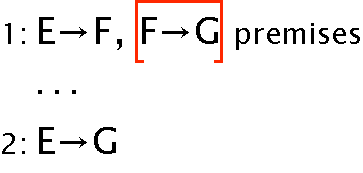
\includegraphics[scale=0.5]{pics/hypothesisselection}}}}
\quad
\subfigure[conclusion selection]{
  \label{fig:conclusionselection}
  \parbox[b]{100pt}{\centering\fbox{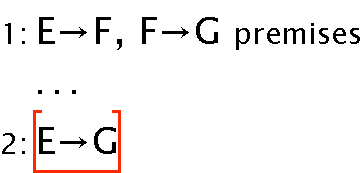
\includegraphics[scale=0.5]{pics/conclusionselection}}}}
\quad
\subfigure[hypothesis and conclusion]{
  \label{fig:hypothesisandconclusion}
  \parbox[b]{100pt}{\centering\fbox{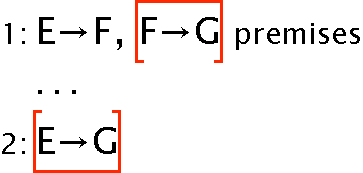
\includegraphics[scale=0.5]{pics/hypothesisandconclusion}}}}
\quad
\subfigure[multi-hypothesis selection]{
  \label{fig:multipleselection}
  \parbox[b]{100pt}{\centering\fbox{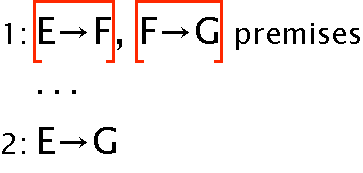
\includegraphics[scale=0.5]{pics/multipleselection}}}}
\caption{Formula selection by mouse click}
\end{figure}

\section{Formula selection}
\label{sec:formulaselection}

Formula selection is made with a single click (left-click on a multi-button mouse). You click on a formula --- a \emph{hypothesis} above the line of dots or a \emph{conclusion} below the dots --- and Jape highlights your selection with an enclosing red box. If you click on a hypothesis you get a downward-facing box as in \figref{hypothesisselection}; if you click on a conclusion you get an upward-facing box as in \figref{conclusionselection}. You can select both a hypothesis and a conclusion, as in \figref{hypothesisandconclusion}.

Clicking on the background --- a white part of the proof window --- cancels all your selections.

Simple clicks will let you select one conclusion and one hypothesis at a time. Normally a second hypothesis click cancels the first, but if you hold down the Shift key while you click you can select more than one hypothesis, as shown in \figref{multipleselection}. And then, also using the Shift key whilst clicking, you can cancel individual formula selections.

There is no way of selecting more than one conclusion at a time.

\begin{figure}
\centering
\subfigure[Proof attempt with intermediate hypothesis/conclusion formula]{
  \label{fig:ambiguousformula}
  \parbox[b]{130pt}{\centering\fbox{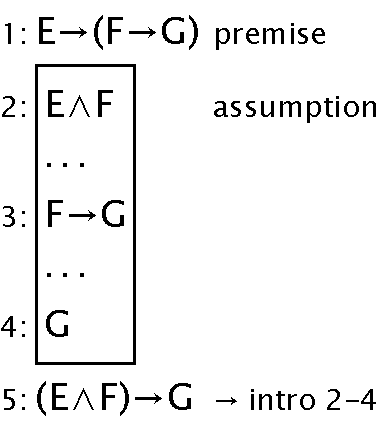
\includegraphics[scale=0.5]{pics/ambiguousformula}}}}
\quad
\subfigure[top-half click selects as conclusion]{
  \label{fig:ambiguousconclusion}
  \parbox[b]{130pt}{\centering\fbox{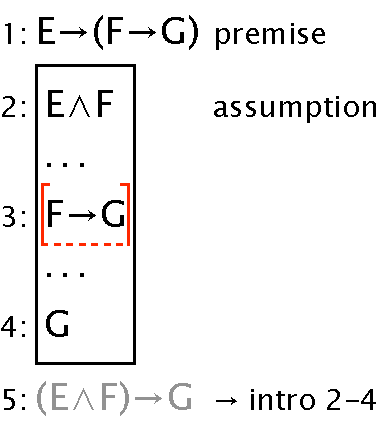
\includegraphics[scale=0.5]{pics/ambiguousconclusion}}}}
\quad
\subfigure[bottom-half click selects as hypothesis]{
  \label{fig:ambiguoushypothesis}
  \parbox[b]{130pt}{\centering\fbox{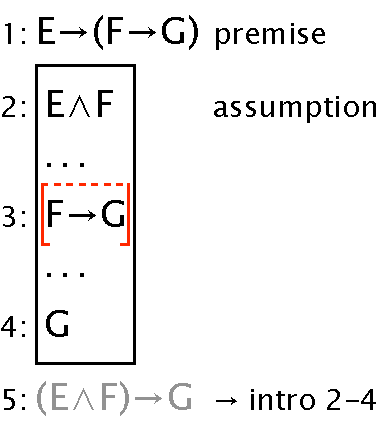
\includegraphics[scale=0.5]{pics/ambiguoushypothesis}}}}
\caption{Ambiguous conclusion/hypothesis selection}
\end{figure}

\subsection{Ambiguous formulae click both ways}

In \figref{ambiguousformula} there are open conclusions on lines 3 and 4, each preceded by a line of dots to show that there's work to be done. Lines 1 and 2 aren't conclusions, and can only be used as hypotheses to prove lines 3 and 4. Line 5 can't be used at all: it's a proved conclusion. Line 4 can only be a conclusion and not a hypothesis, because there's nothing below it in the box. But line 3 is ambiguous: it has to be proved as a conclusion, perhaps using lines 1 and 2, and it can be used as a hypothesis to prove line 4. 

Ambiguous formulae like $F->G$ on line 3 of \figref{ambiguousformula} can be selected in two ways. If you click on the \emph{top half} of the formula you get a box open at the top --- i.e. a conclusion selection --- with a dotted line across the bottom, as shown in \figref{ambiguousconclusion}. If you click on the \emph{bottom half} you get a box open at the bottom --- i.e. a hypothesis selection --- with a dotted line across the top, as shown in \figref{ambiguoushypothesis}.

\subsection{Greying-out}

When you select a hypothesis you can only make a step towards conclusions below you and in the same box as the hypothesis you clicked. When you select a conclusion you can only make a backward step towards hypotheses above you and in the same box or enclosing boxes. Jape greys out all the formulae you can't use, to help you see what's going on, as shown by line 5 in figures \ref{fig:ambiguousconclusion} and \ref{fig:ambiguoushypothesis}. 

If you click on a greyed-out formula Jape cancels your current selection(s). If you click on a conclusion that's already been used up (one which isn't immediately below a line of dots) then Jape greys it out and cancels all your selections.\footnote{This was once a bug. Now it's become a feature, because I rather like it.}

\begin{figure}
\centering
\subfigure[subformula selection]{
  \label{fig:singlesubformulaselection}
  \parbox[b]{150pt}{\centering\fbox{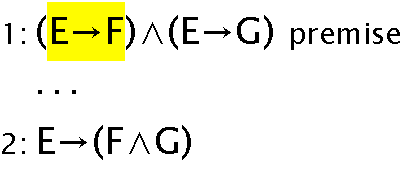
\includegraphics[scale=0.5]{pics/singlesubformulaselection}}}}
\quad
\subfigure[multiple-subformula selection]{
  \label{fig:multiplesubformulaselection}
  \parbox[b]{150pt}{\centering\fbox{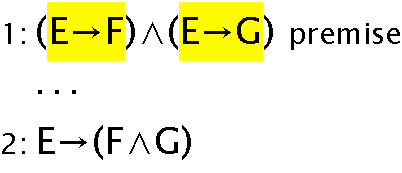
\includegraphics[scale=0.5]{pics/multiplesubformulaselection}}}}
\caption{Subformula selection by option/alt/middle-press-and-drag}
\end{figure}

\section{Subformula selection}
\label{sec:subformulaselection}

Occasionally you need to tell Jape to focus on part of a formula. You do this by a press-and-drag gesture:
\begin{itemize}
\item with a three-button mouse, middle-press-and-drag;
\item otherwise by holding the Alt shift (sometimes labelled 'option') during a press-and-drag.
\end{itemize}
Jape highlights the subformula you've selected by changing the background colour to yellow, as shown in \figref{singlesubformulaselection}. 

If you hold down the add-a-selection shift key (ctrl on Windows and Linux, command on MacOS X) you can make more than one subformula selection, as shown in \figref{multiplesubformulaselection}. Using the same key combination, you can cancel and/or modify subformula selections you've already made.

Jape restricts subformula selections to well-formed subformulae, as you can discover by experiment. That means that if you option/alt/middle-click on a connective or a quantifier, a whole subformula is highlighted. If you option/alt/middle-click on a name, only that name is highlighted.

Option/alt/middle-clicking or pressing on a new subformula cancels all other subformula selections, unless you hold down the add-a-selection shift key (Command on MacOS, Ctrl on other systems). Option/alt/middle-clicking on the background --- a white part of the proof window --- cancels all your subformula selections.

Formula and subformula selections are independent: you can have one without the other, or both, or neither. Cancelling one kind of selection doesn't cancel the other. 

\section{Dragging}

In the disproof pane --- see \chapref{disproof} --- you can drag formulae, tiles, worlds and lines around to make a diagram. You do it by press-and-drag (on a multi-button mouse, left-press-and-drag). Illustrations are given in \chapref{disproof}.


\chapter{Backward and forward steps}
\begin{figure}
\centering
\parbox[b]{200pt}{\centering
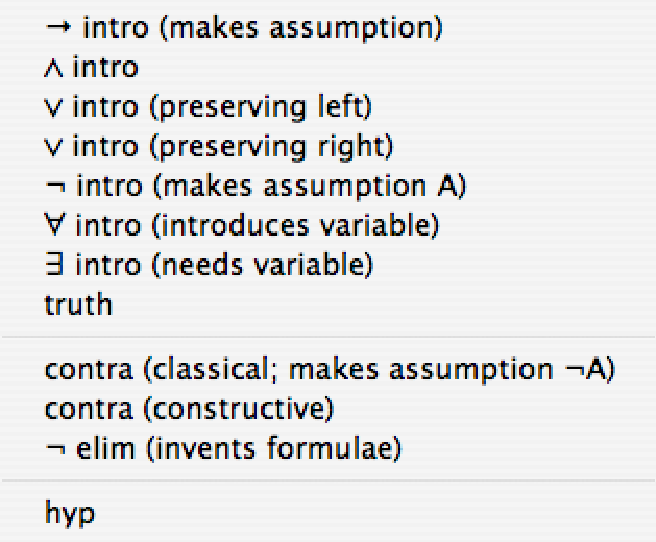
\includegraphics[scale=0.6]{pics/backwardmenu}
\caption{Backward menu}
\label{fig:backwardmenu}}
\qquad
\parbox[b]{200pt}{\centering
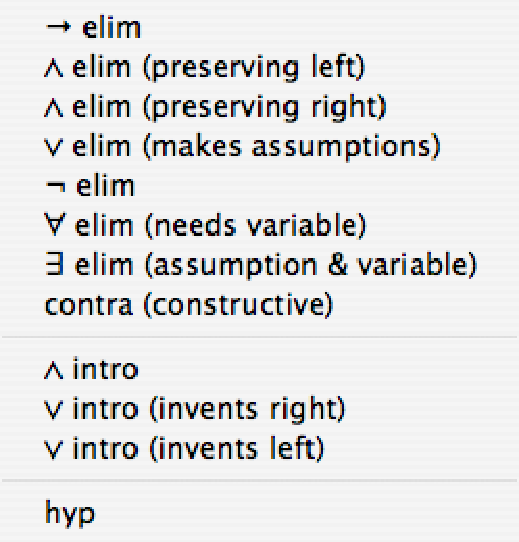
\includegraphics[scale=0.6]{pics/forwardmenu}
\caption{Forward menu}
\label{fig:forwardmenu}}
\end{figure}

Because we read proofs forward, top-to-bottom, forward steps are easiest to understand and most proof novices prefer working forwards. But lots of proofs are difficult working forwards, and some are almost impossibly difficult. To make proofs in Jape you need to be able to make backward steps as well, and I've gone to some trouble to force you to recognise the fact. In the Backward menu, shown in \figref{backwardmenu}, the first group of steps above the line work best backwards and the group below that line can be made to work backward if you try hard. The Forward menu, in \figref{forwardmenu}, similarly shows steps that work well forward before ones that work forward only with difficulty. `hyp' is hard to classify, so it appears in both menus.

To make a step you select one or more formulae and choose a step from the Backward or Forward menu. The selections you need to make depend on the step you choose, and are detailed in the descriptions of the steps in later chapters, but in general for a forward step you must choose a hypothesis and for a backward step an open (unproved) conclusion.

\begin{figure}
\centering
\subfigure[before]{
  \label{fig:two-selectionforwardstepbefore}
  \parbox[b]{200pt}{\centering\fbox{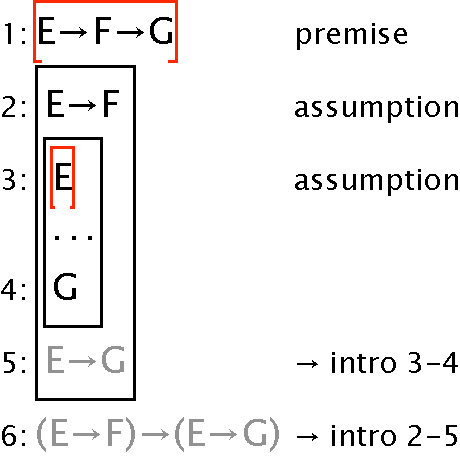
\includegraphics[scale=0.5]{pics/two-selectionforwardstepbefore}}}}
\qquad
\subfigure[after]{
  \label{fig:two-selectionforwardstepafter}
  \parbox[b]{200pt}{\centering\fbox{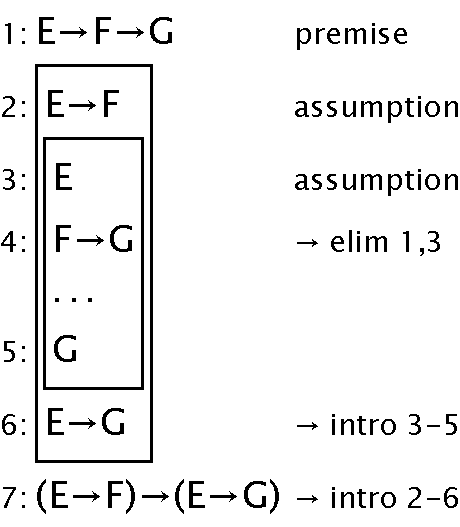
\includegraphics[scale=0.5]{pics/two-selectionforwardstepafter}}}}
\caption{A sample forward step}
\label{fig:two-selectionforwardstep}
\end{figure}
\section{Making a forward step}

Before you make a forward step you must always select a hypothesis formula. Depending on the kind of step, you may have to select more than one hypothesis: for details, see the description of the step later in this manual --- or just try it and see what happens!

You can also select a conclusion as well, if you want to. Some steps require a conclusion selection: you can look up the step in this manual or you can try it out and see what happens. 

Once you have made your selection(s), choose your step from the Forward menu.

Jape writes the result of the step --- the consequent deduced from the antecedent(s) you selected -- just below your selection(s). For example, \figref{two-selectionforwardstep} shows an $->$ elim step with two hypothesis selections. The consequent is line 4 in the `after' picture. Notice that the justification of the step is written against the consequent.

\begin{figure}
\centering
\subfigure[hypothesis only selected]{
  \label{fig:hypselectedignoringtargetbefore}
  \parbox[b]{200pt}{\centering\fbox{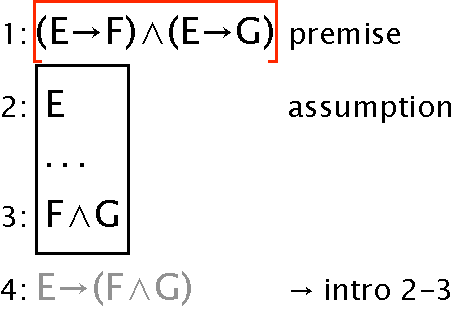
\includegraphics[scale=0.5]{pics/hypselectedignoringtargetbefore}}}}
\qquad
\subfigure[consequent below hypothesis]{
  \label{fig:hypselectedignoringtargetafter}
  \parbox[b]{200pt}{\centering\fbox{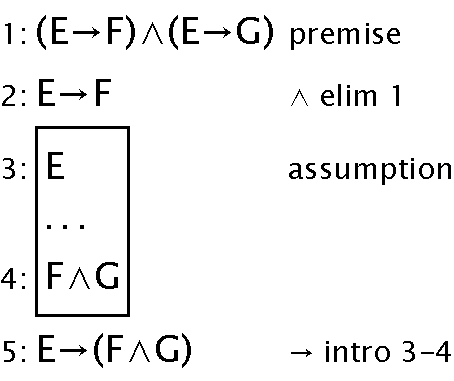
\includegraphics[scale=0.5]{pics/hypselectedignoringtargetafter}}}}
\caption{A forward step without a target conclusion}
\label{fig:hypselectedignoringtarget}
\end{figure}
\begin{figure}
\centering
\subfigure[hypothesis and conclusion selected]{
  \label{fig:hypselectedwithtargetbefore}
  \parbox[b]{200pt}{\centering\fbox{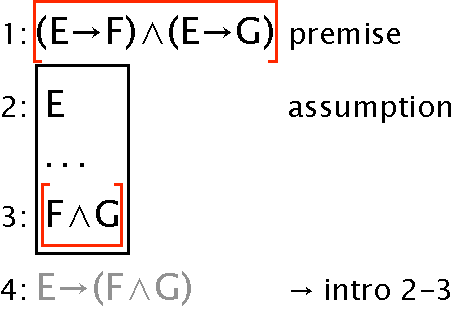
\includegraphics[scale=0.5]{pics/hypselectedwithtargetbefore}}}}
\qquad
\subfigure[consequent above conclusion]{
  \label{fig:hypselectedwithtargetafter}
  \parbox[b]{200pt}{\centering\fbox{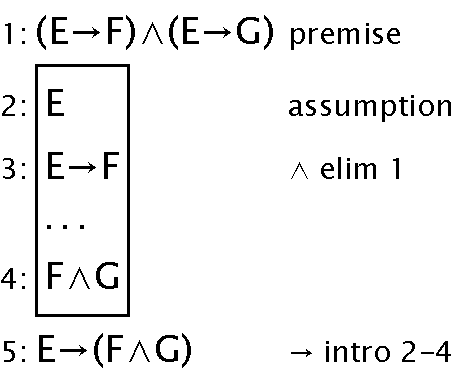
\includegraphics[scale=0.5]{pics/hypselectedwithtargetafter}}}}
\caption{A forward step with a target conclusion}
\label{fig:hypselectedwithtarget}
\end{figure}

\subsection{Selecting a target conclusion}

Normally Jape writes the result of a forward step just after 
the hypothesis selection. Sometimes that may not be convenient, 
and it may be tidier to write it lower down the proof, just above 
a conclusion you are working towards.

In \figref{hypselectedignoringtargetbefore} only the hypothesis on line 1 is selected. A forward step --- in this case ``$@$ elim (ignoring right)'' --- puts its consequent just below the selected hypothesis, as shown in \figref{hypselectedignoringtargetafter}.

If you select a target conclusion as well, as in \figref{hypselectedwithtargetbefore}, the same step will put its consequent before the line of dots above the selected conclusion, as shown in \figref{hypselectedwithtargetafter}.

\subsection{What can go wrong with a forward step?}

When Jape can't make a forward step it's for one of the following reasons. In all cases you'll get an error message which explains the problem.
\begin{enumerate}
\item \emph{No selected hypothesis}. \\
If you don't select a hypothesis formula, you can't make a forward step.

\item \emph{Not enough selections}.\\
Some steps need more than a single hypothesis selection. 

\item \emph{Wrong hypothesis shape}.\\
Most forward steps apply to a particular shape of hypothesis formula. If you select the wrong shape, you can't make the step.

\begin{figure}
\centering
\subfigure[before: hypothesis and conclusion selected]{
  \label{fig:velimneedstargetconclusionbefore}
  \parbox[b]{200pt}{\centering\fbox{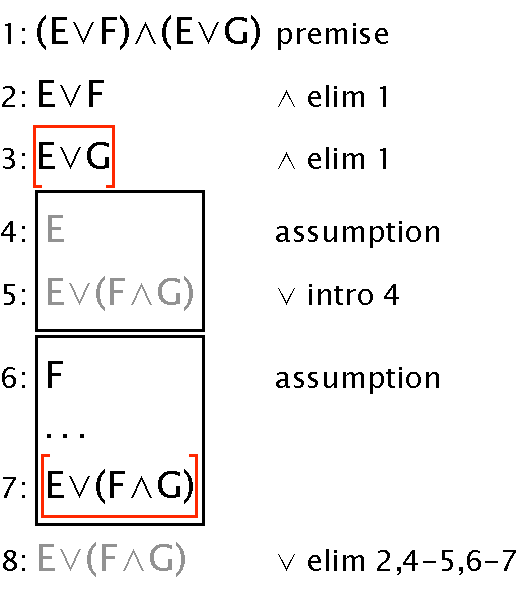
\includegraphics[scale=0.5]{pics/velimneedstargetconclusionbefore}}}}
\qquad
\subfigure[after: argument by cases outlined]{
  \label{fig:velimneedstargetconclusionafter}
  \parbox[b]{200pt}{\centering\fbox{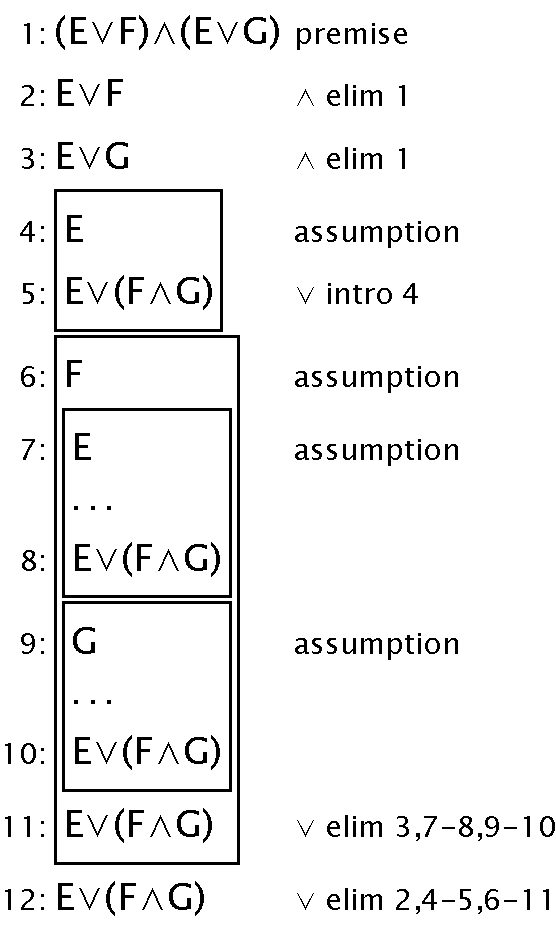
\includegraphics[scale=0.5]{pics/velimneedstargetconclusionafter}}}}
\caption{$|$ elim needs a target conclusion}
\label{fig:velimneedstargetconclusion}
\end{figure}

\item \emph{No target conclusion}.\\
Two forward steps --- $|$ elim, $|*$ elim --- need a conclusion selection as well as a hypothesis, because the consequent can't be calculated from the antecedents. Jape writes the result of the step just above the target conclusion, and writes the justification next to the selected consequent. For example, see the $|$ elim step 
in \figref{velimneedstargetconclusion}. The result of the step (there's quite a lot of it!) is written above line 7 of the `before' state, to form lines 7 to 10 of the `after' state.

%\item \emph{Nowhere to go}.

%When you select a hypothesis, Jape greys-out all the open (unproved) 
%conclusions except the ones that can make use of the hypothesis. 
%If there aren't any reachable open conclusions, Jape won't let you make 
%the forward step (because what use could you make of the result?). 
%In \figref{forwardstepnotarget} there are no open conclusions which can make 
%use of line 2 (there is an open conclusion on line 8, but it's greyed-out because 
%it is in another box and line 2 is irrelevant to it).

%\begin{figure}
%\begin{center}
%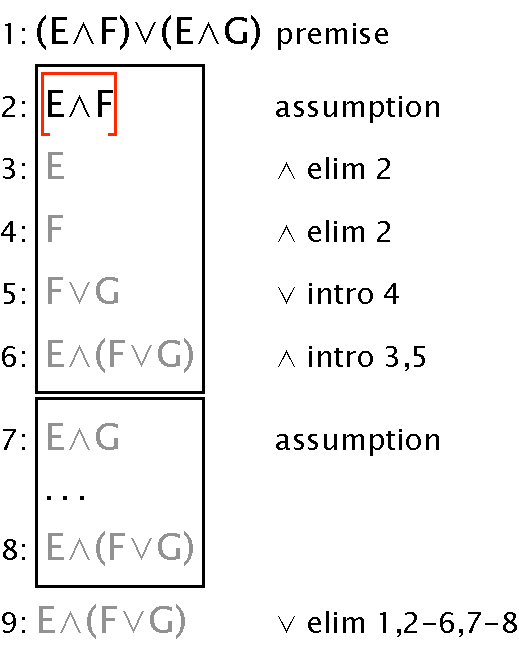
\includegraphics[scale=0.5]{pics/forwardstepnotarget}
%\caption{Hypothesis selection with no open conclusion}
%\label{fig:forwardstepnotarget}
%\end{center}
%\end{figure}

\end{enumerate}


\begin{figure}
\centering
\subfigure[conclusion selected]{
  \label{fig:concselectedforbackwardstep}
  \parbox[b]{200pt}{\centering\fbox{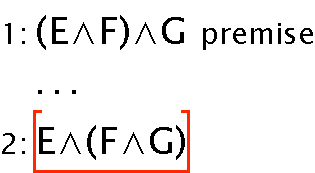
\includegraphics[scale=0.5]{pics/concselectedforbackwardstep}}}}
\qquad
\subfigure[two new conclusion antecedents]{
  \label{fig:concselectedforbackwardstepresult}
  \parbox[b]{200pt}{\centering\fbox{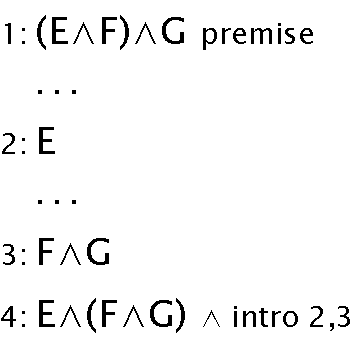
\includegraphics[scale=0.5]{pics/concselectedforbackwardstepresult}}}}
\caption{A sample backward step}
\label{fig:samplebackwardstep}
\end{figure}
\begin{figure}
\centering
\subfigure[conclusion selected]{
  \label{fig:concselectedforbackwardstep2}
  \parbox[b]{200pt}{\centering\fbox{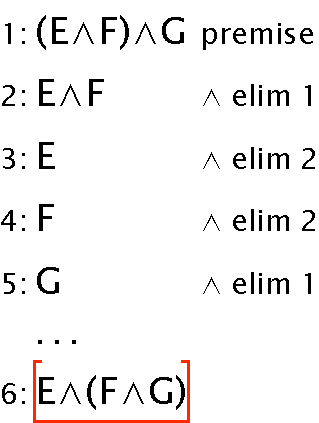
\includegraphics[scale=0.5]{pics/concselectedforbackwardstep2}}}}
\qquad
\subfigure[one hypothesis, one conclusion antecedent]{
  \label{fig:concselectedforbackwardstep2result}
  \parbox[b]{200pt}{\centering\fbox{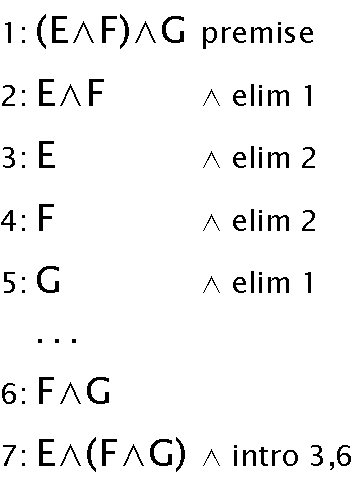
\includegraphics[scale=0.5]{pics/concselectedforbackwardstep2result}}}}
\caption{A sample backward step with a relevant hypothesis}
\label{fig:samplebackwardstepwithhyp}
\end{figure}

\section{Making a backward step}

Backward steps work on an open conclusion --- a line without a justification, written just below a line of three dots. They may prove it completely, if Jape can find hypotheses to match the antecedents, or the antecedents may become unproved conclusions. For example, \figref{concselectedforbackwardstep} shows an open conclusion selection, and \figref{concselectedforbackwardstepresult} shows the effect of a backward $@$ intro step, where each antecedent has become a new open conclusion. \Figref{concselectedforbackwardstep2} shows the same conclusion selected when there are more hypothesis formulae available, and in \figref{concselectedforbackwardstep2result} only one open conclusion is generated because line 3 matches the antecedent of the $@$ intro step.

In every case the justification of the step is written next to the selected conclusion, the consequent of the step.

\subsection{What can go wrong with a backward step?}

\begin{enumerate}
\item \emph{Wrong conclusion shape}.\\
Each backward step, except for contra, applies to a particular shape of consequent formula. If you select the wrong shape, you  can't make the step.

\begin{figure}
\centering
\subfigure[$E$ is the consequent]{
  \label{fig:concselectiondisambiguatesA}
  \parbox[b]{200pt}{\centering\fbox{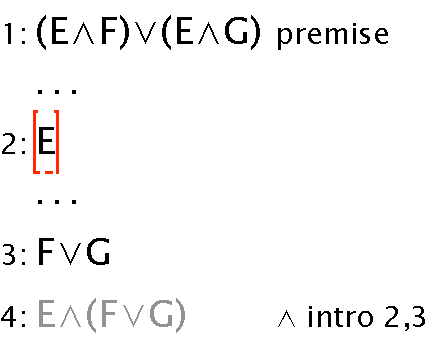
\includegraphics[scale=0.5]{pics/concselectiondisambiguatesA}}}}
\qquad
\subfigure[$F|G$ is the consequent]{
  \label{fig:concselectiondisambiguatesB}
  \parbox[b]{200pt}{\centering\fbox{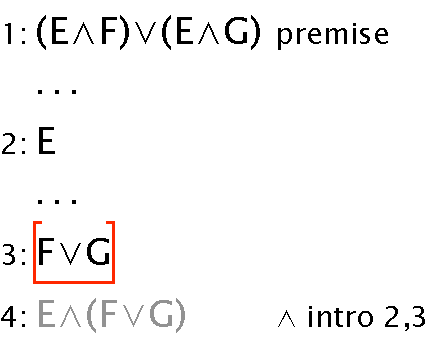
\includegraphics[scale=0.5]{pics/concselectiondisambiguatesB}}}}
\caption{Conclusion selection to tell Jape where to work}
\label{fig:concselectiondisambiguates}
\end{figure}

\item \emph{No selected consequent.}\\
If there is more than one unproved conclusion, Jape doesn't try to choose between them. In \figref{concselectedforbackwardstepresult}, for example, Jape wouldn't know where to apply a backward step. Selecting an unproved conclusion, as in \figref{concselectiondisambiguates}, resolves the ambiguity. (Notice in \figref{concselectiondisambiguatesA} that line 2 is an ambiguous hypothesis/conclusion formula, selected as a conclusion by clicking on it's top half.)\\

\item \emph{Hypothesis selected}.\\
Backward steps (except for $|*$ intro) don't need and can't make use of a selected hypothesis formula. 

\end{enumerate}

\section{Steps which don't need a selection}

If there is only one formula in the proof that can be selected 
as a hypothesis, it would be annoying to be told to select it 
before you can make a forward step. If there's only one unproved 
conclusion in the proof, it would be annoying to be told to select 
that to make a backward step. If the only possible target conclusion 
is on the next line to the hypothesis, it would be annoying to 
be told to select it when a step needs a target. So in all those 
cases Jape lets you get away without selection, and does the 
obvious thing.


\chapter{Rules of thumb for proof search}

Rules of thumb\footnote{An inch was originally defined as the width 
of an adult male thumb, so a `rule of thumb' is an approximate 
measure, then (by punning `rule'=measurer) an approximate guide.\\
There is a Greek word `heuristic' for rule-of-thumb, but I 
prefer the old English. 

Some people object to the English phrase 
because there was once a folk tradition in England that a man 
could legally beat his wife with a stick no thicker than his 
thumb, and it was popularly called rule of thumb. (There's 
a reference, for example, in E.P. Thompson's \textit{Customs in Common}.) The tradition 
was repulsive and mistaken, but (a) it's been forgotten, 
except by historians, and (b) the `approximate guide' reading 
predates it.} are guesswork, approximate guides that don't always 
work. Proof search is much easier if you recognise some simple principles.

\begin{enumerate}
\item Almost all the rules work on the \emph{shape} of a hypothesis 
or consequent formula. Use the shape as a guide to help you choose 
a rule.

\item Use rules that introduce assumptions into the proof \emph{as 
early as possible}. Those rules are: 
\begin{itemize}
\item $->$ intro backwards (for the assumption);
\item $|$ elim forwards (for the assumptions);
\item $!$ intro backwards (for the assumption);
\item $@*$ intro backwards (for the variable);
\item $|*$ elim forwards (for the variable and the assumption).
\end{itemize}

\item $|$ intro works backwards better than it does forwards; but 
since it throws away half the conclusion you apply it to, use 
it very carefully and as late as possible.

\item $!$ elim works better forwards than it does backwards, 
once the contradictory formulae have been revealed.

\item If you use $!$ elim backwards, look for a hypothesis 
to unify with the unproved conclusion $!\_B$ (a negated 
unknown).

\item Classical contra --- `proof by contradiction' --- can be used as 
a last resort in any situation. It introduces an assumption, 
and doesn't mind what shape the consequent is. (Constructive 
contra is just as applicable, but since it doesn't introduce 
an assumption, it isn't usually much help.)

\item If Jape won't let you make the proof, you're \emph{doing it wrong}. 
There aren't any bugs in Jape's treatment of Natural Deduction, 
and all the proofs in the Conjectures and Classical conjectures 
panels are possible --- I've done them all. Similarly, all the 
ones in the Invalid conjectures panel are impossible (they are 
included so that you can disprove them --- see \chapref{disproof}).

\item Don't be afraid to Undo and Redo to search alternative routes to proof. Jape permits multiple Undos and corresponding Redos.

\end{enumerate}

\section{Look at the shape of the formula}

There is a general principle: logical steps 
in Natural Deduction almost always simplify a formula, removing 
a connective ($->$, $@$, $|$ or $!$) or a quantifier ($@*$ 
or $|*$) and breaking the formula into its constituent parts. Persuasion 
(intro) rules do that working backwards, and use (elim) rules 
do it forwards. To choose a rule, look for the main connective 
(or the quantifier) in an unproved conclusion or a hypothesis, 
and use the rule which works on that connective (or quantifier).

The way that rules match formulae is so nearly mechanical 
that I could have set Jape up to choose the relevant rule 
when you merely double-click on a formula. Because I want you 
to learn about Natural Deduction and not just the use of the 
mouse, I've been grandad-ish and set it up so that you have to 
choose the rules for yourself.

\chapter{The steps summarised}

\section{$->$ steps}

\begin{figure}
\centering
\subfigure[$E->(F->G)$ selected]{
  \label{fig:arrowintrobackwardbefore}
  \parbox[b]{200pt}{\centering\fbox{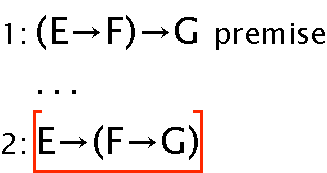
\includegraphics[scale=0.5]{pics/arrowintrobackwardbefore}}}}
\qquad
\subfigure[hypothetical argument outlined]{
  \label{fig:arrowintrobackwardafter}
  \parbox[b]{200pt}{\centering\fbox{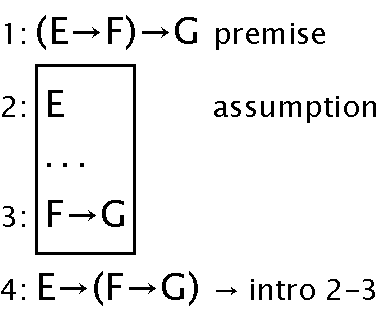
\includegraphics[scale=0.5]{pics/arrowintrobackwardafter}}}}
\caption{$->$ intro backward}
\label{fig:arrowintrobackward}
\end{figure}

You can use $->$ intro backward by selecting a $A->B$ hypothesis. See \figref{arrowintrobackward}, for example. Notice that the step introduces a new assumption and therefore a new box (and that's why it should be used early).

\begin{figure}
\centering
\subfigure[$E$ and $E->F$ selected]{
  \label{fig:arrowelimforwardbefore}
  \parbox[b]{200pt}{\centering\fbox{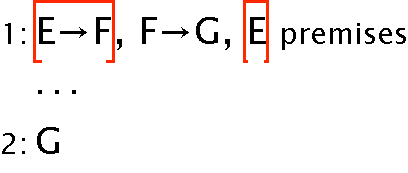
\includegraphics[scale=0.5]{pics/arrowelimforwardbefore}}}}
\qquad
\subfigure[consequent $F$ deduced]{
  \label{fig:arrowelimforwardafter}
  \parbox[b]{200pt}{\centering\fbox{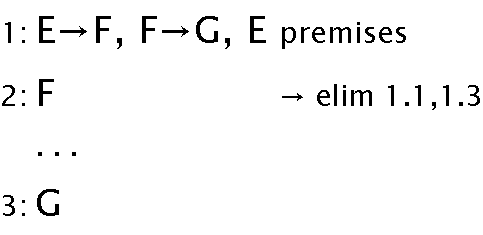
\includegraphics[scale=0.5]{pics/arrowelimforwardafter}}}}
\caption{$->$ elim forward}
\label{fig:arrowelimforward}
\end{figure}

You can use $->$ elim forward by selecting a $A$ hypothesis and a $A->B$ hypothesis, as shown by the trivial example in \figref{arrowelimforward}. (Shift-click to select the second hypothesis: if you select the wrong thing either cancel it with a shift-click or click on the background to cancel all your selections, and start again.)

\begin{figure}
\centering
\subfigure[$F->G$ and target conclusion selected]{
  \label{fig:-arrowelimhalfbackwardbefore}
  \parbox[b]{200pt}{\centering\fbox{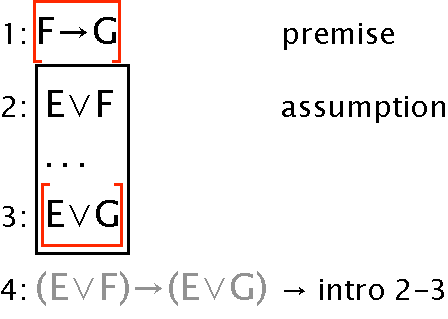
\includegraphics[scale=0.5]{pics/arrowelimhalfbackwardbefore}}}}
\qquad
\subfigure[consequent $G$ deduced from new open conclusion $F$]{
  \label{fig:arrowelimhalfbackwardafter}
  \parbox[b]{200pt}{\centering\fbox{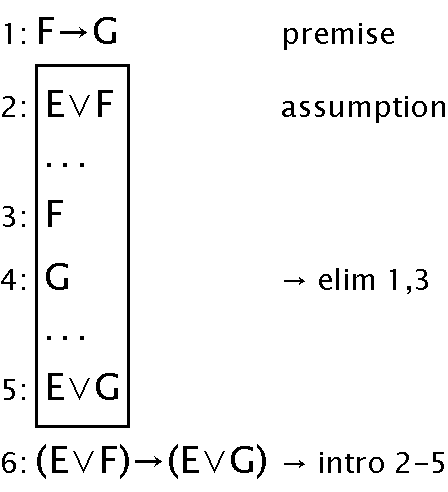
\includegraphics[scale=0.5]{pics/arrowelimhalfbackwardafter}}}}
\caption{$->$ elim half backward, half forward}
\label{fig:arrowelimhalfbackward}
\end{figure}

You can also use $->$ elim half-forward, half-backward if you select a $A->B$ hypothesis and a target conclusion and apply ``$->$ elim'' from the Forward menu. Jape writes a new conclusion $A$ followed by a consequent $B$, as shown in \figref{arrowelimhalfbackward}. It's a half-backward step because it introduces a new conclusion.

$->$ intro forward is just daft, and Jape won't attempt it. $->$ elim backward is possible, but it introduces unknowns and there's no real advantage, so I don't let Jape try.
 
\section{$@$ steps}

You can use $@$ intro backward to generate antecedent conclusion lines, as shown in figures \ref{fig:samplebackwardstep} and \ref{fig:samplebackwardstepwithhyp} on page \pageref{fig:samplebackwardstep}. Select a conclusion, make the step. I strongly recommend using $@$ intro backward rather than forward.

You can use $@$ elim forward, picking out either the left or the right subformula, as shown in figures \ref{fig:hypselectedignoringtarget} and \ref{fig:hypselectedwithtarget} on page \pageref{fig:hypselectedignoringtarget}.

\begin{figure}
\centering
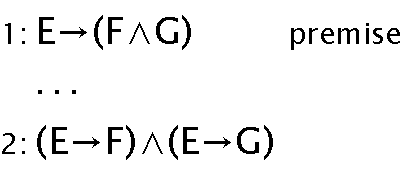
\includegraphics[scale=0.5]{pics/@introbackwardsworks}
\caption{$@$ intro backwards needed}
\label{fig:@introbackwardsworks}
\end{figure}

$@$ intro forward is also possible: select two hypothesis formulae to be the antecedents. But it's usually easier backwards: really it is. \Figref{@introbackwardsworks}, for example, is easy if the first step is $@$ intro backwards --- you have two things to prove and you have to prove them separately --- and impossible almost any other way.

$@$ elim backwards is possible, but for some reason or other I didn't include it (and I'm sure I had a good reason, so I'm not going to add it now).

\begin{figure}
\centering
\subfigure[before: conclusion selected]{
  \label{fig:vintrobackwardsiseasyA}
  \parbox[b]{200pt}{\centering\fbox{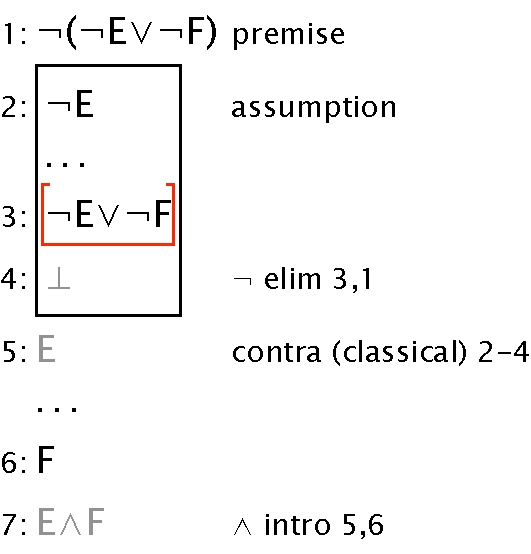
\includegraphics[scale=0.5]{pics/vintrobackwardsiseasyA}}}}
\qquad
\subfigure[after: uncertainty resolved]{
  \label{fig:vintrobackwardsiseasyB}
  \parbox[b]{200pt}{\centering\fbox{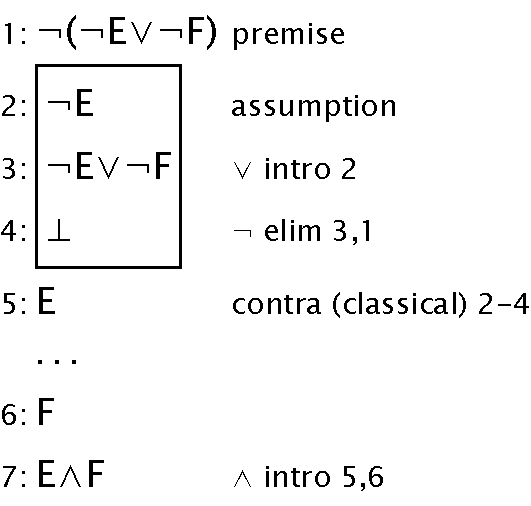
\includegraphics[scale=0.5]{pics/vintrobackwardsiseasyB}}}}
\caption{$|$ intro backwards is easy}
\label{fig:vintrobackwardsiseasy}
\end{figure}

\begin{figure}
\centering
\subfigure[before: hypothesis selected]{
  \label{fig:vintroforwardsgeneratesunknownA}
  \parbox[b]{200pt}{\centering\fbox{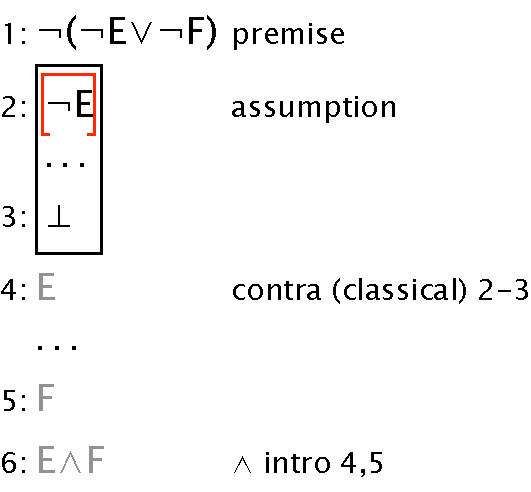
\includegraphics[scale=0.5]{pics/vintroforwardsgeneratesunknownA}}}}
\qquad
\subfigure[after: `unknown' formula introduced]{
  \label{fig:vintroforwardsgeneratesunknownB}
  \parbox[b]{200pt}{\centering\fbox{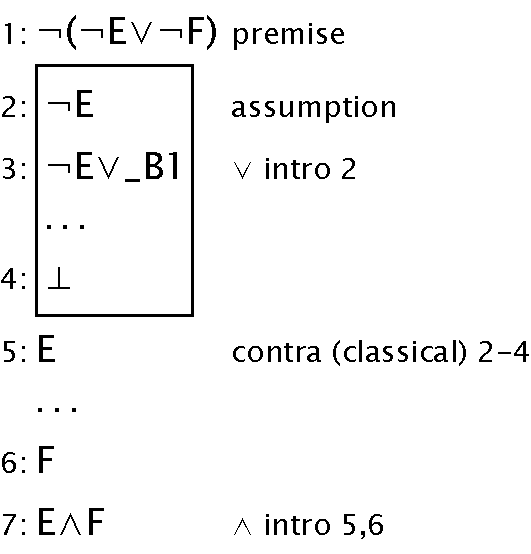
\includegraphics[scale=0.5]{pics/vintroforwardsgeneratesunknownB}}}}
\caption{$|$ intro forwards generates an unknown}
\label{fig:vintroforwardsgeneratesunknown}
\end{figure}

\section{$|$ steps}

Because $|$ elim forwards implements argument by cases, and because the consequent $C$ can't be deduced from the $A|B$ antecedent, it generates big proof changes from a small gesture. That frightens novices, but be brave, because $|$ elim is one of the rules that generates assumptions, so you have to use it as early as possible in a proof.

$|$ intro backwards is destructive --- it throws away half a conclusion --- so you use it as \emph{late} as possible, even though it's very easy to use.

You use $|$ elim forwards by selecting a hypothesis which fits $A|B$, an open conclusion $C$ (if there's only one available conclusion, and if its on the line below the hypothesis, Jape will let you off the conclusion selection) and ``$|$ elim'' from the Forward menu. See \figref{velimneedstargetconclusion} on page \pageref{fig:velimneedstargetconclusion}, for example. Note that the boxes representing the $A$ leads to $C$ and $B$ leads to $C$ arguments (lines 7-8 and 9-10 in \figref{velimneedstargetconclusionbefore}, for example) are written just above the selected conclusion $C$, and the justification is (of course) written against the selected conclusion.

$|$ intro is easy to use backwards: select an open conclusion, decide which half to keep and which to throw away, and apply the corresponding step (``$|$ intro (preserving left)'' or ``$|$ intro (preserving right)'') from the Backward menu. See \figref{vintrobackwardsiseasy}, for example.

For some reason that I've forgotten, I was persuaded to allow $|$ intro forward. I rather regret it, because this isn't a step for novices to use. But, if you must: you select a hypothesis, decide which half of the consequent it has to be, and apply the corresponding step (``$|$ intro (inventing left)'' or ``$|$ intro (inventing right)'') from the Forward menu. The step always invents an unknown, as illustrated in \figref{vintroforwardsgeneratesunknown} by an ``inventing right'' step, and you have to deal with the unknown somehow (see \chapref{unknowns} for suggestions).

If unknowns frighten you, don't use $|$ intro forwards (the easy way to solve the proof problem in \figref{vintroforwardsgeneratesunknown}, for example, is $!$ elim forwards from line 1 with target conclusion line 4, producing \figref{vintrobackwardsiseasyA}; then $|$ intro backwards preserving left produces \figref{vintrobackwardsiseasyB}). 

$|$ elim backwards would be possible, but not for novices, so I didn't allow it.

\begin{figure}
\centering
\subfigure[before: hypothesis $!(E|F)$ and target conclusion selected]{
  \label{fig:!elimforwardsiseasyA}
  \parbox[b]{200pt}{\centering\fbox{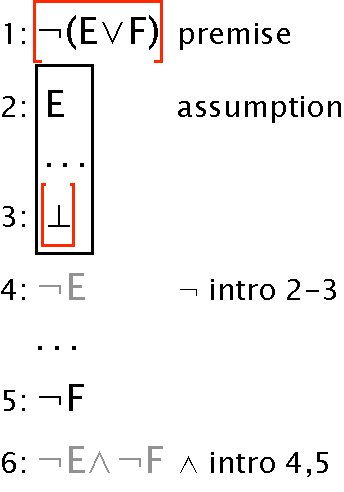
\includegraphics[scale=0.5]{pics/!elimforwardsiseasyA}}}}
\qquad
\subfigure[after: conclusion $E|F$ generated]{
  \label{fig:!elimforwardsiseasyB}
  \parbox[b]{200pt}{\centering\fbox{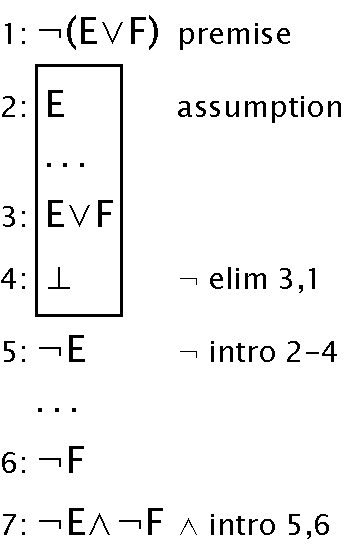
\includegraphics[scale=0.5]{pics/!elimforwardsiseasyB}}}}
\caption{$!$ elim forwards is easy}
\label{fig:!elimforwardsiseasy}
\end{figure}

\begin{figure}
\centering
\subfigure[before: conclusion $!F$ selected]{
  \label{fig:!introbackwardsiseasyA}
  \parbox[b]{200pt}{\centering\fbox{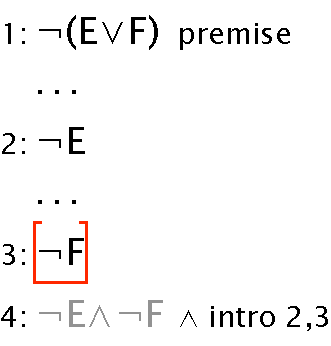
\includegraphics[scale=0.5]{pics/!introbackwardsiseasyA}}}}
\qquad
\subfigure[after: contradiction argument outlined]{
  \label{fig:!introbackwardsiseasyB}
  \parbox[b]{200pt}{\centering\fbox{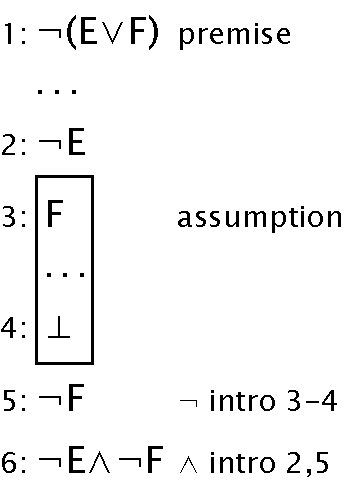
\includegraphics[scale=0.5]{pics/!introbackwardsiseasyB}}}}
\caption{$!$ intro backwards is very easy}
\label{fig:!introbackwardsiseasy}
\end{figure}

\begin{figure}
\centering
\subfigure[before: conclusion $\bot$ selected]{
  \label{fig:!elimbackwardsisharderA}
  \parbox[b]{200pt}{\centering\fbox{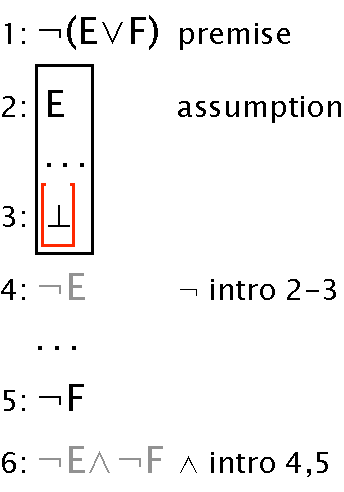
\includegraphics[scale=0.5]{pics/!elimbackwardsisharderA}}}}
\qquad
\subfigure[after: unknown $\_\mathit{B1}$ invented, and two conclusions generated]{
  \label{fig:!elimbackwardsisharderB}
  \parbox[b]{200pt}{\centering\fbox{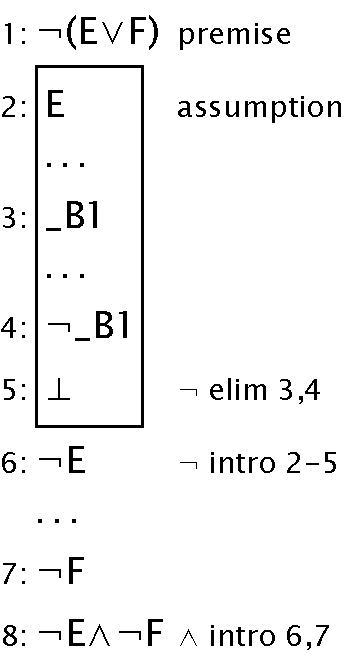
\includegraphics[scale=0.5]{pics/!elimbackwardsisharderB}}}}
\caption{$!$ elim backwards is harder}
\label{fig:!elimbackwardsisharder}
\end{figure}

\section{$!$ steps}

$!$ elim works best forwards, $!$ intro backwards.

To use $!$ elim forwards, select a hypothesis $!A$, or two hypotheses $!A$ and $A$ and choose ``$!$ elim'' from the Forward menu. You can select a target conclusion too, if you like. The step generates a consequent $\bot$, plus a conclusion $A$, if you only select one hypothesis. See \figref{!elimforwardsiseasy}, for example.

To use $!$ intro backwards, select an open conclusion $!B$ and ``$!$ intro'' from the Backward menu. See \figref{!introbackwardsiseasy}, for example.

It's possible to use $!$ elim backwards, if you select an open conclusion $\bot$. It generates an unknown $\_B$ and two new open conclusions $!\_B$ and $!\_B$, as illustrated in \figref{!elimbackwardsisharder}. It's usually easier to do it forwards, though.

$!$ intro forwards doesn't make much sense, so I didn't allow it.

\begin{figure}
\centering
\subfigure[before: conclusion $E|!E$ selected]{
  \label{fig:classicalcontrastepA}
  \parbox[b]{200pt}{\centering\fbox{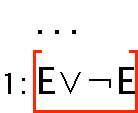
\includegraphics[scale=0.5]{pics/classicalcontrastepA}}}}
\qquad
\subfigure[after: contradiction argument outlined]{
  \label{fig:classicalcontrastepB}
  \parbox[b]{200pt}{\centering\fbox{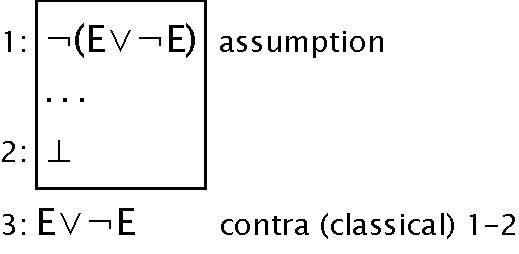
\includegraphics[scale=0.5]{pics/classicalcontrastepB}}}}
\caption{A sample classical contradiction step}
\label{fig:classicalcontrastep}
\end{figure}

\begin{figure}
\centering
\subfigure[before: hypothesis $\bot$ and target conclusion selected]{
  \label{fig:constructivecontraforwardsA}
  \parbox[b]{200pt}{\centering\fbox{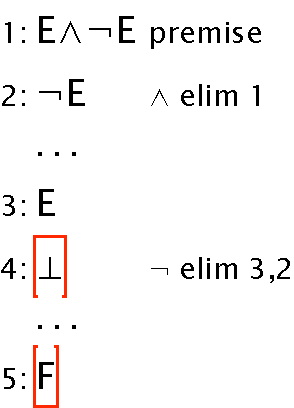
\includegraphics[scale=0.5]{pics/constructivecontraforwardsA}}}}
\qquad
\subfigure[after: conclusion `proved']{
  \label{fig:constructivecontraforwardsB}
  \parbox[b]{200pt}{\centering\fbox{\includegraphics[scale=0.5]{pics/constructivecontraforwardsB}}}}
\caption{A sample constructive contradiction step}
\label{fig:constructivecontraforwards}
\end{figure}

\section{$\bot$ (contradiction) steps}

Classical contra is a hard rule to use (there ought to be a blues song about that), but you know you are going to have to use it for some problems. It only works backwards. Constructive contra is easier if you use it forwards.

To use classical contra, select an open conclusion $A$ and choose ``contra (classical)'' from the Backward menu. It creates a hypothetical contradiction argument with assumption $!A$, as shown in \figref{classicalcontrastep}.

To use constructive contra forwards, select a $\bot$ hypothesis and an open conclusion, and choose ``contra (constructive)'' from the Forward menu. See \figref{constructivecontraforwards}, for example.

Constructive contra backwards is destructive: it throws away whatever conclusion it is applied to. But you can do it if you want to. Classical contra forwards would be absurd.

\section{$\top$ (truth) step}

You can always prove $\top$ as an open conclusion: select it and apply ``truth'' from the Backward menu. And that's all you can do with $\top$: no forward step is possible.

\begin{figure}
\centering
\subfigure[before: $@*x.!R(x)$ conclusion selected]{
  \label{fig:forallintrobackwardsA}
  \parbox[b]{200pt}{\centering\fbox{\includegraphics[scale=0.5]{pics/forallintrobackwardsA}}}}
\qquad
\subfigure[after: generalised proof outline introduced, with private variable $i$]{
  \label{fig:forallintrobackwardsB}
  \parbox[b]{200pt}{\centering\fbox{\includegraphics[scale=0.5]{pics/forallintrobackwardsB}}}}
\caption{A $@*$ intro step backwards}
\label{fig:forallintrobackwards}
\end{figure}

\begin{figure}
\centering
\subfigure[before: $@*x.(R(x)@S(x))$ and $\protect\<actual> i$ hypotheses selected]{
  \label{fig:forallelimforwardsA}
  \parbox[b]{200pt}{\centering\fbox{\includegraphics[scale=0.5]{pics/forallelimforwardsA}}}}
\qquad
\subfigure[after: $R(i)@S(i)$ consequent deduced]{
  \label{fig:forallelimforwardsB}
  \parbox[b]{200pt}{\centering\fbox{\includegraphics[scale=0.5]{pics/forallelimforwardsB}}}}
\caption{A $@*$ elim step forwards}
\label{fig:forallelimforwards}
\end{figure}

\section{$@*$ steps}
\var{i1,i2}
$@*$ intro works backwards, $@*$ elim forwards. $@*$ intro is worth using early, because it introduces a variable. The privacy condition on the $@*$ intro step won't usually bother you, because Jape always invents a new variable ($i$, $\<i1>$, $\<i2>$, and so on).

To use $@*$ intro backwards, select an open conclusion $@*x.P(x)$ and choose ``$@*$ intro'' from the Backward menu. Jape builds the outline of the generalised proof, as illustrated in \figref{forallintrobackwards}. 

To use $@*$ elim forwards, you must select a hypothesis $@*x.P(x)$ and also $\<actual> j$, then choose ``$@*$ elim'' from the Forward menu. The effect is illustrated in \figref{forallelimforwards}.

%If your proof attempt contains unknowns then $@*$ intro may generate provisos: see \secref{provisos}.

\begin{figure}
\centering
\subfigure[before: $|*x.!R(x)$ hypothesis and target conclusion $\bot$ selected]{
  \label{fig:existselimforwardsA}
  \parbox[b]{200pt}{\centering\fbox{\includegraphics[scale=0.5]{pics/existselimforwardsA}}}}
\qquad
\subfigure[after: generalised proof outline introduced, with private variable $i$]{
  \label{fig:existselimforwardsB}
  \parbox[b]{200pt}{\centering\fbox{\includegraphics[scale=0.5]{pics/existselimforwardsB}}}}
\caption{An $|*$ elim step forwards}
\label{fig:existselimforwards}
\end{figure}

\begin{figure}
\centering
\subfigure[before: $|*x.!R(x)$ conclusion and $\protect\<actual> i$ hypothesis selected]{
  \label{fig:existsintrobackwardsA}
  \parbox[b]{200pt}{\centering\fbox{\includegraphics[scale=0.5]{pics/existsintrobackwardsA}}}}
\qquad
\subfigure[after: $!R(i)$ antecedent deduced]{
  \label{fig:existsintrobackwardsB}
  \parbox[b]{200pt}{\centering\fbox{\includegraphics[scale=0.5]{pics/existsintrobackwardsB}}}}
\caption{An $|*$ elim step backwards}
\label{fig:existsintrobackwards}
\end{figure}

\section{$|*$ steps}
$|*$ intro works backwards, $|*$ elim forwards. $|*$ elim is worth using early, because it introduces a variable. The privacy condition on the $|*$ elim step won't usually bother you, because Jape always invents a new variable ($i$, $\<i1>$, $\<i2>$, and so on).

To use $|*$ elim forwards, you must select a hypothesis $|*x.P(x)$ and also a target conclusion, and then choose ``$|*$ elim'' from the Forward menu. The justification is written next to the target conclusion, and a generalised proof outline is introduced, as illustrated in \figref{existselimforwards}.

To use $|*$ intro backwards, you must select a conclusion $|*x.P(x)$ and also a hypothesis $\<actual> j$, and then choose ``$|*$ intro'' from the Backward menu. The effect is illustrated in \figref{existsintrobackwards}.

%If your proof attempt contains unknowns then $|*$ elim may generate provisos: see \secref{provisos}.

\chapter{Unknowns, hyp and Unify}
\label{chap:unknowns}
\var{B1}

When James Aczel looked at novices learning logic with Jape, he pointed out that they found \emph{incomplete steps} quite disconcerting. Incomplete steps are ones that let you leave out important information so that you can fill it in later, when you've discovered what it ought to be. You might be allowed to leave out the variable in an $|*$ intro step, for example, and fill it in later. 

Jape uses \emph{unknowns} --- names starting with an underscore, like $\_\<B1>$ --- to stand for formulae which can be filled in later. Even though James persuaded me to eliminate almost all incomplete steps from my treatment of natural deduction, my users pleaded with me to allow some. So it is possible to introduce unknowns into a Jape proof, and because of that it's necessary to know how to get rid of them again.

To understand what follows you have to recognise the distinction between \emph{formula selection} (red box round a conclusion or a hypothesis formula) and \emph{subformula selection} (yellow background behind part or all of a conclusion or hypothesis formula). Note, in particular, that a subformula selection that encompasses a complete formula is \emph{not} the same thing as a formula selection.

\begin{figure}
\centering
\subfigure[before: $|*x.!R(x)$ hypothesis selected]{
  \label{fig:orintroforwardsA}
  \parbox[b]{200pt}{\centering\fbox{\includegraphics[scale=0.5]{pics/orintroforwardsA}}}}
\qquad
\subfigure[after: unknown $\_\protect\<B1>$ introduced in consequent]{
  \label{fig:orintroforwardsB}
  \parbox[b]{200pt}{\centering\fbox{\includegraphics[scale=0.5]{pics/orintroforwardsB}}}}
\caption{An $|$ intro step forwards}
\label{fig:orintroforwards}
\end{figure}

\begin{figure}
\centering
\subfigure[before: conclusion is $\bot$]{
  \label{fig:notelimbackwardsA}
  \parbox[b]{200pt}{\centering\fbox{\includegraphics[scale=0.5]{pics/notelimbackwardsA}}}}
\qquad
\subfigure[after: unknown $\_\protect\<B1>$ introduced in antecedents]{
  \label{fig:notelimbackwardsB}
  \parbox[b]{200pt}{\centering\fbox{\includegraphics[scale=0.5]{pics/notelimbackwardsB}}}}
\caption{A $!$ elim step backwards}
\label{fig:notelimbackwards}
\end{figure}

\section{Introducing an unknown}

$|$ elim backwards takes a formula with an $|$ connective and throws away half of it, because from $A$ you can prove $A|B$, and from $B$ you can prove $A|B$. Some obsessively-forward reasoners wanted me to allow $|$ intro forwards, and just to spite them I did: it's there in the Forward menu, under the line. \Figref{orintroforwards} shows how you can deduce $A|\_B$ from $A$ by choosing ``$|$ intro (inventing right)'' from the Forward menu.

$!$ elim backwards is another good way to get an unknown, illustrated in \figref{notelimbackwards}. There's only one unknown in the proof, but it occurs twice.

These are by no means the only way to introduce unknowns into a proof. One very interesting way is to select a conclusion, choose ``Text command'' from the File menu, type ``apply cut'' and press return. You will get an unknown, intermediate between the hypotheses and your conclusion. I leave you to work out how useful that can be.

\begin{figure}
\centering
\subfigure[before: conclusion $\bot$ selected, subformula $!R(x)$ selected]{
  \label{fig:notelimbackwardswithsubformulaA}
  \parbox[b]{200pt}{\centering\fbox{\includegraphics[scale=0.5]{pics/notelimbackwardswithsubformulaA}}}}
\qquad
\subfigure[after: $!R(x)$ used in antecedents of $!$ elim]{
  \label{fig:notelimbackwardswithsubformulaB}
  \parbox[b]{200pt}{\centering\fbox{\includegraphics[scale=0.5]{pics/notelimbackwardswithsubformulaB}}}}
\caption{A $!$ elim step backwards with subformula selection}
\label{fig:notelimbackwardswithsubformula}
\end{figure}

\section{Avoiding unknowns by subformula selection}

If you know beforehand what should go in place of the unknown, you can tell Jape what to use at the time you make an $|$ intro or $!$ elim step, by subformula selection (alt/option/middle-press-and-drag over the formula or subformula you want to use). \Figref{notelimbackwardswithsubformula} shows an example: note that the hypothesis is \emph{not} selected, but $!R(x)$ is subformula-selected.

\begin{figure}
\centering
\subfigure[before: subformulae $|*x.!R(x)$ and $\_\protect\<B1>$ selected]{
  \label{fig:unifyreplacesunknownA}
  \parbox[b]{200pt}{\centering\fbox{\includegraphics[scale=0.5]{pics/unifyreplacesunknownA}}}}
\qquad
\subfigure[after: instances of $\_\protect\<B1>$ replaced by $|*x.!R(x)$]{
  \label{fig:unifyreplacesunknownB}
  \parbox[b]{200pt}{\centering\fbox{\includegraphics[scale=0.5]{pics/unifyreplacesunknownB}}}}
\caption{Effect of a Unify command}
\label{fig:unifyreplacesunknown}
\end{figure}

\section{Eliminating an unknown with Unify}

If you have an unknown in your proof, and a subformula somewhere in the proof which you want to use to replace the unknown, then subformula selection and the ``Unify'' command from the Edit menu will do the job. You subformula-select two or more subformulae which you want to make the same by replacing unknowns (command/control-alt/option/middle-press-and-drag is the gesture you need to make more than one subformula selection). \Figref{unifyreplacesunknown} shows an example. Note that there are no formula selections in \figref{unifyreplacesunknownA}, only subformula selections.

\begin{figure}
\centering
\subfigure[before: hypothesis $!|*x.!R(x)$ and conclusion $!\_\protect\<B1>$ selected]{
  \label{fig:hypreplacesunknownA}
  \parbox[b]{200pt}{\centering\fbox{\includegraphics[scale=0.5]{pics/hypreplacesunknownA}}}}
\qquad
\subfigure[after: instances of $\_\protect\<B1>$ replaced by $|*x.!R(x)$]{
  \label{fig:hypreplacesunknownB}
  \parbox[b]{200pt}{\centering\fbox{\includegraphics[scale=0.5]{pics/hypreplacesunknownB}}}}
\caption{Effect of \texttt{hyp} on an unknown}
\label{fig:hypreplacesunknown}
\end{figure}

\section{Eliminating an unknown with \texttt{hyp}}

The \texttt{hyp} step is really just a cloak for the Unify command: make this selected conclusion the same as this selected hypothesis (or these selected hypotheses). For example see \figref{hypreplacesunknown}. Note that making $!|*x.!R(x)$ the same as $!\_\<B1>$ means making $|*x.!R(x)$ the same as $\_\<B1>$.

\begin{figure}
\centering
\parbox[b]{250pt}{\centering\includegraphics[scale=0.5]{pics/proofwithproviso}
\caption{Proof with proviso}
\label{fig:proofwithproviso}}
\quad
\parbox[b]{200pt}{\centering\fbox{\includegraphics[scale=0.5]{pics/disallowedunification}}
\caption{Preparation for proviso-violating unification}
\label{fig:disallowedunification}}
\end{figure}

\begin{figure}
\centering
\includegraphics[scale=0.45]{pics/NOTINerrormessage}
\caption{Jape's reason for rejecting unification step}
\label{fig:NOTINerrormessage}
\end{figure}

\section{Provisos and the privacy condition}
\label{sec:provisos}

Recall that the $@*$ intro and $|*$ elim steps use a variable --- $i$, $\<i1>$, $\<i2>$, ... --- for use privately within a generalised proof. If a proof attempt doesn't include unknowns, Jape can enforce the privacy condition easily: simply use a variable that isn't in use already, anywhere in the proof. If there are unknowns about, things aren't so simple: Jape has to ensure that you don't unify that unknown with a formula that uses the private variable, because that would violate the privacy condition. 

\Figref{proofwithproviso} shows what happens when Jape has to invent a variable and there is an unknown in the proof. It must prohibit the possibility that the formula $\_\<B1>$ includes the variable $i$: it does this with the \emph{proviso} ``$i \text{ NOTIN } \_\<B1>$'' in the \emph{proviso pane} below the proof. \Figref{disallowedunification} shows preparation for an attempt to violate the proviso with a Unify command (making $\_\<B1>$, which appears outside the box, the same as $R(i)$ inside the box). \Figref{NOTINerrormessage} shows the error message that Jape generates when you try the unification.


%
%It's often more convenient to eliminate unknowns after they have 
%arrived in the proof. One easy way to do this is to use the Unify 
%command in the Edit menu. You text-select as many formulae as 
%you want, and Jape tries to make them all the same by replacing 
%unknowns with ordinary formulae.\footnote{\tab The technical name for 
%this process is \textit{unification}, hence the name of the command.} 
%Suppose you have

%\begin{figure}[htbp]
%\begin{center}
%\includegraphics[width=2.361in, height=2.153in]{natural_deduction_manualFig74.pict}
%\caption{natural_deduction_manualFig74.pict about here.}
%\end{center}
%\end{figure}

%
%We want to make $!$F and \_B1 the same. Text-select them 
%both

%\begin{figure}[htbp]
%\begin{center}
%\includegraphics[width=2.361in, height=2.153in]{natural_deduction_manualFig75.pict}
%\caption{natural_deduction_manualFig75.pict about here.}
%\end{center}
%\end{figure}

%
%and choose Unify from the Edit menu: the unknown disappears and 
%is replaced by the formula.

%\begin{figure}[htbp]
%\begin{center}
%\includegraphics[width=2.319in, height=2.153in]{natural_deduction_manualFig76.pict}
%\caption{natural_deduction_manualFig76.pict about here.}
%\end{center}
%\end{figure}

%
%\textbf{{\large 9.4 Eliminating an unknown with a hyp step}}

%
%Instead of unifying by text selection, we sometimes tell Jape 
%to unify a hypothesis formula with a consequent formula, using 
%the hyp step which is on both Forward and Backward menus.

%
%Back to an earlier example:

%\begin{figure}[htbp]
%\begin{center}
%\includegraphics[width=2.361in, height=1.653in]{natural_deduction_manualFig77.pict}
%\caption{natural_deduction_manualFig77.pict about here.}
%\end{center}
%\end{figure}

%
%Now when using $!$ elim backwards, as we had to do in this 
%example, the rules of thumb say that we should look for a hypothesis 
%which will unify with the negated unknown $!$\_B1. There 
%is only one negated hypothesis, on line 1. Try that. Click on 
%line 1 and on line 3

%\begin{figure}[htbp]
%\begin{center}
%\includegraphics[width=2.361in, height=1.653in]{natural_deduction_manualFig78.pict}
%\caption{natural_deduction_manualFig78.pict about here.}
%\end{center}
%\end{figure}

%
%and choose hyp from either the Forward or the Backward menu. 
%The effect is to unify the two formulae. Jape changes the justification 
%of the $@$ intro step to point to the assumption, throws away 
%the unnecessary conclusion, and the proof looks like this:

%\begin{figure}[htbp]
%\begin{center}
%\includegraphics[width=2.361in, height=1.250in]{natural_deduction_manualFig79.pict}
%\caption{natural_deduction_manualFig79.pict about here.}
%\end{center}
%\end{figure}

%
%After that it's up to you (hint: it's ok to try $|$ intro backwards 
%now).


\chapter{Disproof}
\label{chap:disproof}
%\newpage

%\begin{center}
%11. Disproof

%
%\end{center}

%Disproof uses forcing semantics. To make a disproof of an assertion, 
%you build a situation just like the ones in the lecture notes: 
%a structure of blobs (worlds) connected by lines, with formulae 
%attached to the worlds. Just as Jape ensures that you can't make 
%an invalid proof step, so it ensures that you can only build 
%a valid situation: it adds and removes formulae, and even lines, 
%to ensure that you stay within the rules.

%
%Each time you make a situation Jape evaluates it and shows you 
%whether you have a counter-example. It explains the evaluation 
%by showing you information about subformulae inside the sequent 
%you are checking. You can move about the situation, looking at 
%forcing in different worlds. You can even check the status of 
%a subproof, if you are worried that you are stuck in a dead end.

%
%In the lecture notes I emphasise the way that a failed proof 
%search can guide a search for a disproof. Most of the examples 
%which follow use this approach. On the other hand, I know that 
%people learn a lot by just trying things out, exploring what 
%is possible, and in an appendix I describe what is possible

%
%\textbf{{\large 11.1 Getting started with disproof}}

%
%\textit{The disproof pane}

%
%Disproof takes place in a separate pane of the window, at the 
%top. At any stage of a proof you can choose Disprove from the 
%Edit menu, the disproof pane will appear at the top of the window 
%if it isn't already there, and a basic situation --- an isolated 
%empty world --- will be drawn, with the sequent you are trying 
%to disprove below it. (Note the semantic turnstile \`{I}, pronounced 
%`models'.)

%
%\textit{Choosing a sequent}

%
%For simplicity, use Disprove without selecting a conclusion: 
%then the sequent in the disproof pane is the one which started 
%the current proof --- that is, the premises and conclusion of the 
%problem you chose from a conjectures panel. If you select a conclusion, 
%Jape makes a sequent from that conclusion and the formulae above 
%it in the proof that it can call upon.

%
%\textit{Making worlds and lines}

%
%When you start a disproof, there is always a single isolated 
%world. To make more worlds, use the right mouse button to press-and-drag 
%on a world: Jape makes a copy of the world you are dragging and 
%links it to the world you dragged from. (If you drag your new 
%world to a position level with or below the old world, Jape won't 
%make a linking line).

%
%\textit{Moving worlds}

%
%Left press-and-drag moves a world to a new position. Dragging 
%a world level with or below its parent world deletes the linking 
%line.

%
%\textit{Attaching formulae}

%
%Jape gives you a collection of tiles to the right of the disproof 
%pane. You drag a tile (left mouse button) to a world and drop 
%it there. Jape silently adds the same formula to any child worlds, 
%to preserve the monotonicity condition. You can't drop a formula 
%onto a world where it already appears. 

%
%\textit{Individuals and predicates}

%
%Jape gives you tiles for the minimum number of individuals (actual 
%\textit{i} and the like) you need in order to work with the sequent 
%you are disproving. If you need another individual, double-click 
%(left mouse button) on an `individual' tile: double-clicking actual 
%\textit{i}, for example, will give you actual \textit{i1}.

%
%In a similar way, Jape gives you a minimum number of instantiated 
%predicate tiles (
%$R\left( i\right) $
%, 
%$S\left( j,k\right) $
% and the like). If you need a predicate instantiated with a different 
%individual, double-click one of the ones you have: double-clicking 

%$R\left( i\right) $
%, for example, when you have actual \textit{i} and actual \textit{i1}, 
%will give you 
%$R\left( i1\right) $
%. Jape will refuse if there aren't any unused individuals (you 
%have to get a new individual first); it will give you a choice 
%if there is more than one possibility.

%
%\textit{Deleting worlds, lines and attached formulae}

%
%You can't (this is a deficiency). You have to use Undo Disproof 
%Step from the Edit menu, and improvise. Sorry.

%
%\textit{Completing a disproof}

%
%Jape underlines forced premises and conclusions. When all the 
%premises are underlined, but the conclusion isn't, you have a 
%disproof. You use Done from the Edit menu and Jape records the 
%disproof in the panel you got the problem with.\footnote{\tab Jape ought 
%to notice when you have a classical proof and a constructive 
%disproof. It doesn't (this is a deficiency).}

%
%\textit{Printing disproofs}

%
%You can't (this is a deficiency). If you know how to print a 
%snapshot of a window, please tell me.

%
%\textbf{{\large 11.2 A trivial classical disproof}}

%
%Classical counter-examples (see the lecture notes) use a single 
%world. Sometimes the isolated empty world is a counter-example. 
%Consider 
%$E\rightarrow \left( F\rightarrow G\right) \,\,\left( E\rightarrow F\right)
%\rightarrow G$
%, an assertion which suggests that it doesn't matter if we bracket 
%implications to the left rather than the right. It isn't provable 
%(though it works in the other direction: see the Conjectures 
%panel). Proof of the counter-assertion, or disproof of the assertion, 
%needs a counter-example.

%
%Start a proof of the assertion (it's top of the Invalid Conjectures 
%panel) and immediately press Disprove. You will see, in the disproof 
%pane, a picture like this:

%\begin{figure}[htbp]
%\begin{center}
%\includegraphics[width=2.236in, height=1.417in]{natural_deduction_manualFig88.pict}
%\caption{natural_deduction_manualFig88.pict about here.}
%\end{center}
%\end{figure}

%
%The isolated empty world is shown ringed with a red selection 
%(since it's the only world, it must be selected); the tiles at 
%the right are the formulae that can be dragged onto a world. 
%The sequent at the bottom is shown with a semantic turnstile, 
%to emphasise that this window is about the model not the formal 
%proof system.

%
%Jape gives you information about forcing using violet,\footnote{\tab Well 
%it's violet as I designed it, to make a useful contrast with 
%the red colour used for selection. You can change it in the preferences 
%if you want to.} black and grey. Violet means forced, black means 
%unforced (and grey we shall come to later). In this particular 
%example there is a a violet line underlining the premise, and 
%no underlining of the conclusion. Each occurrence of the basic 
%facts \textit{E}, \textit{F} and \textit{G} is black. Reading from left to right 
%the first three arrows are violet, and the last is black. All 
%the brackets are violet.

%
%By underlining the premise, Jape is showing you that it is forced. 
%By not underlining the conclusion, it is showing you that it 
%is \textit{not} forced. So the simplest of all situations --- the isolated 
%empty world --- is a counter-example to the assertion, a situation 
%in which the premise is forced but the conclusion isn't. One 
%counter-example destroys an assertion: the isolated empty world 
%disproves 
%$E\rightarrow \left( F\rightarrow G\right) \,\,\left( E\rightarrow F\right)
%\rightarrow G$
%, and, since natural deduction is sound, thereby disproves 
%$E\rightarrow \left( F\rightarrow G\right) \,\,\left( E\rightarrow F\right)
%\rightarrow G$
%.\\
%By emphasising and de-emphasising brackets, basic facts and operators, 
%Jape is pointing to an explanation of just why this is a counter-example. 
%None of \textit{E}, \textit{F} or \textit{G} is forced in this situation, so 
%all of them are show in black. And then, because we never come 
%across \textit{F}, 
%$F\rightarrow G$
% is forced, and so its arrow is shown in violet together with 
%its enclosing brackets.. Because we never come across \textit{E}, 

%$E\rightarrow \left( F\rightarrow G\right) $
% is forced too, and its arrow is shown violet --- and then, because 
%it's the whole premise, the premise is underlined.

%
%On the right, 
%$E\rightarrow F$
% is forced because we never come across \textit{E}, so its arrow and 
%brackets are violet. But since 
%$E\rightarrow F$
% is forced at the root world but \textit{G} isn't, 
%$\left( E\rightarrow F\right) \rightarrow G$
% is \textit{not} forced, and its arrow is black. And then, since the 
%conclusion isn't forced, it isn't underlined.

%
%If you drag tiles to the selected world, you can upset the applecart. 
%Dragging \textit{E} and dropping it onto the world gives the following:

%\begin{figure}[htbp]
%\begin{center}
%\includegraphics[width=2.236in, height=1.431in]{natural_deduction_manualFig89.pict}
%\caption{natural_deduction_manualFig89.pict about here.}
%\end{center}
%\end{figure}

%
%Now that \textit{E} is forced, both its occurrences in the sequent 
%are violet. The premise is still forced, because wherever we 
%see \textit{E} we see 
%$F\rightarrow G$
%. But now the conclusion is forced also. The black arrow shows 
%that 
%$E\rightarrow F$
% is \textit{not} forced (there's a world which forces \textit{E} but not 
%\textit{F}) and so, by the cunning uncle argument, 
%$\left( E\rightarrow F\right) \rightarrow G$
% \textit{is} forced.

%
%Adding \textit{G} doesn't improve matters:

%\begin{figure}[htbp]
%\begin{center}
%\includegraphics[width=2.236in, height=1.417in]{natural_deduction_manualFig90.pict}
%\caption{natural_deduction_manualFig90.pict about here.}
%\end{center}
%\end{figure}

%
%Getting rid of both of them (use Undo Disproof Step from the 
%Edit menu\footnote{\tab At the time of writing there isn't a way to delete 
%formulae from worlds. There is on the Mac, but that's another 
%story.}) and adding \textit{F} makes an alternative counter-example, 
%as does adding both \textit{E} and \textit{F} (check out the violet and 
%black to see why):\\

%
%\begin{longtable}{|p{2.250in}|p{2.250in}|}
%\hline
%% ROW 1
%{\raggedright } & 
%{\raggedright }\\
%\hline
%\end{longtable}

%
%But of course (!) if you add \textit{G}, everything is ruined again.

%
%\textbf{{\large 11.3 Making a classical disproof}}

%
%Sometimes, as in the example, above, the isolated empty world 
%is a counter-example, and as soon as you ask for a disproof Jape 
%shows you one. More often you have to work a little.

%
%Consider, for example, 
%$\left( E\rightarrow F\right) \rightarrow G\,\,E\wedge \left( F\rightarrow
%G\right) $
%. This has a classical disproof, as it happens. The way you find 
%out that is has is to make a disproof!\footnote{\tab Or you could rely 
%on the fact that it's in the Invalid Conjectures panel...} It 
%isn't the isolated empty world, as Jape will show you at once 
%(the left-hand side isn't forced because 
%$E\rightarrow F$
% is forced, but there is no G; the right-hand side isn't forced 
%because there is no \textit{E}):

%\begin{figure}[htbp]
%\begin{center}
%\includegraphics[width=2.222in, height=1.431in]{natural_deduction_manualFig93.pict}
%\caption{natural_deduction_manualFig93.pict about here.}
%\end{center}
%\end{figure}

%
%Given this much information about the isolated empty world, and 
%with a bit of experience you can see that the left-hand side 
%is forced with a \textit{G}, but the right-hand side isn't (it needs 
%\textit{E} as well). With less experience, or with more complicated 
%examples, it pays to explore the shape of possible proofs first. 
%The first two steps are straightforward:

%\begin{figure}[htbp]
%\begin{center}
%\includegraphics[width=1.722in, height=1.986in]{natural_deduction_manualFig94.pict}
%\caption{natural_deduction_manualFig94.pict about here.}
%\end{center}
%\end{figure}

%
%To make a disproof you only have to break one arm of the proof. 
%This proof attempt seems to suggest that if we had \textit{F} but 
%not \textit{G} we would have a disproof --- but not so, as the disproof 
%pane shows (drag tile \textit{F} onto the root world):

%\begin{figure}[htbp]
%\begin{center}
%\includegraphics[width=2.222in, height=1.431in]{natural_deduction_manualFig95.pict}
%\caption{natural_deduction_manualFig95.pict about here.}
%\end{center}
%\end{figure}

%
%If we work a little harder we can push the proof inside the box 
%to a conclusion (first step select lines 1 and 4 and choose \ensuremath{\rightarrow} 
%elim; the rest is straightforward):

%\begin{figure}[htbp]
%\begin{center}
%\includegraphics[width=1.722in, height=2.708in]{natural_deduction_manualFig96.pict}
%\caption{natural_deduction_manualFig96.pict about here.}
%\end{center}
%\end{figure}

%
%This tells us that premise 
%$\left( E\rightarrow F\right) \rightarrow G$
% does force conclusion 
%$F\rightarrow G$
%. So if we are to avoid forcing 
%$E\wedge \left( F\rightarrow G\right) $
% we have to do it by avoiding forcing \textit{E}. The bridge which 
%might connect line 1 to line 2 starts with classical contra, 
%continues with \ensuremath{\rightarrow} elim and finishes up like this:

%\begin{figure}[htbp]
%\begin{center}
%\includegraphics[width=2.486in, height=2.722in]{natural_deduction_manualFig97.pict}
%\caption{natural_deduction_manualFig97.pict about here.}
%\end{center}
%\end{figure}

%
%We are guaranteed a disproof if we force \textit{G} on its own (to 
%build this disproof remove \textit{F}, if necessary, by using Undo 
%Disproof Step):

%\begin{figure}[htbp]
%\begin{center}
%\includegraphics[width=2.222in, height=1.431in]{natural_deduction_manualFig98.pict}
%\caption{natural_deduction_manualFig98.pict about here.}
%\end{center}
%\end{figure}

%
%Half the conclusion is still forced, of course (!), but we need 
%to force both halves of the \ensuremath{\wedge} connective and we don't 
%force \textit{E}, so this is a counter-example.

%
%\textbf{{\large 11.4 Making a constructive disproof}}

%
%Making disproof is most interesting when there's a classical 
%proof but a constructive disproof: that is, there is a counter-example, 
%but it takes more than a single world to show it.\\
%Consider, for example, 
%$\neg F\rightarrow \neg E\,\,E\rightarrow F$
%. This has a very simple classical proof (try it!) but it doesn't 
%have a constructive proof. Here's as far as you can go with a 
%direct constructive approach:

%\begin{figure}[htbp]
%\begin{center}
%\includegraphics[width=1.528in, height=1.306in]{natural_deduction_manualFig99.pict}
%\caption{natural_deduction_manualFig99.pict about here.}
%\end{center}
%\end{figure}

%
%The box tells you that you will get a counter-example if you 
%add a world which forces \textit{E} but doesn't force \textit{F}. To make 
%that counter-example, choose Disprove from the Edit menu:

%\begin{figure}[htbp]
%\begin{center}
%\includegraphics[width=1.639in, height=0.986in]{natural_deduction_manualFig100.pict}
%\caption{natural_deduction_manualFig100.pict about here.}
%\end{center}
%\end{figure}

%
%Adding \textit{E} to this world doesn't make a counter-example (neither 
%side is forced):

%\begin{figure}[htbp]
%\begin{center}
%\includegraphics[width=1.639in, height=0.986in]{natural_deduction_manualFig101.pict}
%\caption{natural_deduction_manualFig101.pict about here.}
%\end{center}
%\end{figure}

%
%So remove \textit{E} (Undo Disproof Step from the Edit menu) and add 
%a world (right press-and-drag on the root world):

%\begin{figure}[htbp]
%\begin{center}
%\includegraphics[width=1.639in, height=0.986in]{natural_deduction_manualFig102.pict}
%\caption{natural_deduction_manualFig102.pict about here.}
%\end{center}
%\end{figure}

%
%Drop \textit{E} into the new world, and Jape still says no good:

%\begin{figure}[htbp]
%\begin{center}
%\includegraphics[width=2.569in, height=1.903in]{natural_deduction_manualFig103.pict}
%\caption{natural_deduction_manualFig103.pict about here.}
%\end{center}
%\end{figure}

%
%We're not forcing conclusion 
%$E\rightarrow F$
%, but we're not forcing 
%$\neg F\rightarrow \neg E$
% either. Jape shows us a clue: the $!$ connective in 
%$\neg F$
% is violet, so although the root world doesn't force \textit{F} (black) 
%it does force 
%$\neg F$
% (violet connective). It also shows us (black connective) that 
%we aren't forcing 
%$\neg E$
%, so the promise of 
%$\neg F\rightarrow \neg E$
% fails at the root world.

%
%The problem, once again, is that we haven't pushed the proof 
%attempt far enough. Using \ensuremath{\rightarrow} elim, constructive contra 
%and $!$ intro gives us this in the proof pane:

%\begin{figure}[htbp]
%\begin{center}
%\includegraphics[width=2.208in, height=2.708in]{natural_deduction_manualFig104.pict}
%\caption{natural_deduction_manualFig104.pict about here.}
%\end{center}
%\end{figure}

%
%We are told to build a world which forces \textit{E}, and within that 
%force \textit{F}. Forcing \textit{F} at the top world doesn't do the job, 
%so we know we need another world which forces \textit{F}:

%\begin{figure}[htbp]
%\begin{center}
%\includegraphics[width=2.569in, height=1.903in]{natural_deduction_manualFig105.pict}
%\caption{natural_deduction_manualFig105.pict about here.}
%\end{center}
%\end{figure}

%
%Undo Disproof Step gets rid of \textit{F}; then right press-and-drag 
%on the top world gives a new one (notice that Jape automatically 
%includes \textit{E} to preserve monotonicity):

%\begin{figure}[htbp]
%\begin{center}
%\includegraphics[width=2.569in, height=1.903in]{natural_deduction_manualFig106.pict}
%\caption{natural_deduction_manualFig106.pict about here.}
%\end{center}
%\end{figure}

%
%Add \textit{F} to the new top world and the job's done (
%$\neg F$
% is no longer forced, so 
%$\neg F\rightarrow \neg E$
% is cunning-uncle forced; there's a world which forces \textit{E} 
%but not \textit{F} so 
%$E\rightarrow F$
% isn't forced):

%\begin{figure}[htbp]
%\begin{center}
%\includegraphics[width=2.569in, height=1.903in]{natural_deduction_manualFig107.pict}
%\caption{natural_deduction_manualFig107.pict about here.}
%\end{center}
%\end{figure}

%
%\textbf{{\large 11.5 A classical disproof with quantifiers}}

%
%Here is why constructivists need not be afraid of the universal 
%drunk:

%\begin{figure}[htbp]
%\begin{center}
%\includegraphics[width=4.028in, height=1.958in]{natural_deduction_manualFig108.pict}
%\caption{natural_deduction_manualFig108.pict about here.}
%\end{center}
%\end{figure}

%\newpage

%\begin{center}
%12. Using theorems and stating conjectures

%
%\end{center}

%The Apply button in the Conjectures panel lets you use theorems 
%(proved conjectures) just like rules.

%
%ND Jape matches a theorem to a proof by replacing some or all 
%of the names in the theorem. But only some names are replaceable, 
%and it uses a simple lexical convention to help it to decide. 
%Names in sequents fall into one of three classes:

%
%{\textbullet}\tab \textit{variables}: any name starting with \textit{x}, \textit{y}, \textit{z} or 
%\textit{i}, \textit{j}, \textit{k};\\
%{\textbullet}\tab \textit{formulas}: any name starting with \textit{A,} \textit{B}, \textit{C}, 
%\textit{E}, \textit{F}, \textit{G}, \textit{P}, \textit{Q}, \textit{R} or \textit{S}.

%
%Variable names in a theorem sequent can be replaced by any variable, 
%formula names by any formula, constant names by any constant. 
%This means, for example, that E$->$(F$->$G), E \^{E} F$->$G, and (E1$@$E2)$->$(F1$|$F2), 
%E1$@$E1 \^{E} F1$|$F2 are each instances of E$->$F, E \^{E} F.

%
%I use formula names \textit{A}, \textit{B} and \textit{C} in rules, \textit{E}, \textit{F} 
%and \textit{G} in conjectures. I use predicate name \textit{P} in rules, 
%\textit{Q}, \textit{R} and \textit{S} in conjectures.

%
%\textbf{{\large 11.1 Applying theorems}}

%
%You apply a theorem \textit{either} to a consequent \textit{or}  to an 
%hypothesis. At the time of writing this manual, Jape is better 
%at applying theorems to a consequent. So: click on a conclusion 
%and apply the theorem. If the right-hand side of the theorem 
%matches the conclusion, Jape does so. If not, it generates a 
%version of the theorem using unknowns, and you fill in the gaps.

%
%\textbf{{\large 11.2 Stating your own conjectures}}

%
%The (New) button in the Conjectures panel lets you define your 
%own conjectures. It brings up a dialogue box which looks like 
%this:

%\begin{figure}[htbp]
%\begin{center}
%\includegraphics[width=6.625in, height=2.944in]{natural_deduction_manualFig109.pict}
%\caption{natural_deduction_manualFig109.pict about here.}
%\end{center}
%\end{figure}

%
%You type your conjecture as a sequent into the top pane of the 
%box labelled \textsc{conjecture}. The keypad is there so that you 
%don't have to learn Vulcan keyboard grips for connectives, quantifiers 
%or turnstile. When you're ready, press Execute (top left). Unless 
%you've made a mistake, Jape adds your conjecture to the Conjectures 
%panel and selects it, so that you can press Prove to start a 
%proof of it.

%
%To get rid of the dialogue box, press Close (top right). (I don't 
%know what the other buttons do: experiment if you are interested.) 

%

%\textit{Troubleshooting}

%
%When you are stating a conjecture, don't forget to distinguish 
%between the various classes of name (see above). If you use a 
%name which is outside either class, Jape will refuse to accept 
%the conjecture. \\
%If you make a mistake, Jape's response won't be very easy to understand. 
%If you make more than one error, Jape only spots the first.

%\newpage

%\begin{center}
%13. Printing a proof (File menu)

%
%\end{center}

%If you choose Print from the File menu, your proof will automatically 
%be printed, labelled with your username. It's directed to the 
%printer described by your PRINTER environment variable --- the 
%same place that a lpr command will send its output.\footnote{\tab There 
%ought to be a dialogue box to allow you to select a printer, 
%alter the label --- and so on --- before printing. There isn't one 
%at the time of writing. Sorry.}

%
%You may want to do more complicated word-processing things with 
%your proof, and it's possible to save your proof as an EPS (Encapsulated 
%PostScript) file (if you don't know what that is or why you would 
%need it, relax and skip to the next section). This is what you 
%do. Choose \textit{Save proof as}  \textit{Postscript} in the File menu; 
%tell it where to put its output. The output has to be printed 
%with the program /import/jape/jlpr, whose output should be piped 
%to lpr.

%\newpage

%\begin{center}
%14. Saving and restoring your proofs (the File menu)

%
%\end{center}

%On the File menu there are a collection of commands to open, 
%close and save files of logic descriptions and proofs. The \textit{Save} 
%and \textit{Save As} commands will save a file of proofs; \textit{Load 
%a proof (.jp) file} will load them back in. \textit{Quit} exits Jape 
%(same as the go-away button in the top right of the window). 
%Other commands do other things, which I don't explain here.

%
%\textit{Save} and \textit{Save As} will save your completed proofs, and 
%any proofs in progress in the session window, in a file of your 
%choice, using a file-selection dialogue (it's best to save them 
%in files called \textit{somethingorother}.jp). \textit{Load a proof (.jp) 
%file} will load them back again (and it will automatically look 
%for files called \textit{whatsit}.jp, which is why it's best to save 
%proofs in a file with that sort of name). If you have any unsaved 
%proofs when you quit, or any proofs in progress in the session 
%window, Jape will ask you if you want to save them.

%
%If you want to build up a collection of proofs in a file, make 
%sure you reload your old proofs before you start adding to the 
%collection. If you start a new collection and then save it to 
%the same file, ND Jape will --- without checking that it is what 
%you want to do --- overwrite the old collection.

%\newpage

%\begin{center}
%Appendix A: Using the mouse

%
%\end{center}

%ND Jape on X understands various mouse gestures in the proof 
%pane:

%
%{\textbullet}\tab a single \textit{left-button} \textit{click} selects a hypothesis or consequent 
%formula to work on;\\
%{\textbullet}\tab a single \textit{middle-button click} to select a character 
%as an argument to a rule;

%
%{\textbullet}\tab \textit{press and drag} with the \textit{middle button} down to select 
%a sequence of characters as argument to a rule;\\
%{\textbullet}\tab \textit{press and drag} with the \textit{middle button} down over 
%a blank portion of the pane to move the proof within the pane.

%
%In addition, various mouse gestures cancel the effect of some 
%of the above:

%
%{\textbullet}\tab a \textit{left-button click} or \textit{middle-button click} in a blank 
%area of the screen cancels all formula and text selections;\\
%{\textbullet}\tab a \textit{middle-button click} over a text selection cancels 
%it (and, currently, any other text selections in the same formula, 
%but not any in other formulae);

%
%\textit{Single-left-click}

%
%A box is drawn round the formula you clicked on, open at the 
%top (consequent formula) or at the bottom (hypothesis formula), 
%and it becomes a focus of attention for the command you apply. 
%You can select more than one hypothesis, but only a single consequent 
%formula. 

%
%To cancel a selection, left-click it again. Left-clicking in 
%a blank area of the pane cancels all formula and text selections.

%
%\textit{Double-left-click}

%
%Jape can understand double-clicks, but I've programmed ND Jape 
%to ignore them.

%
%\textit{Middle-click and middle-press-and-drag}

%
%If you click the middle button over a character it is text-selected; 
%if you press the middle button over a character, hold it down, 
%and move the mouse left or right, that character and the others 
%you drag over are text-selected; in either case the selected 
%text is highlighted. It looks like this:

%
%\begin{center}
%\includegraphics[width=2.431in, height=0.667in]{natural_deduction_manualFig110.pict}
%\end{center}

%

%To cancel a text selection, middle-click it. Middle clicking 
%in a blank area of the proof pane cancels all text selections.

%\newpage

%\begin{center}
%Appendix B --- Troubleshooting

%
%\end{center}

%\textbf{{\large Problems with windows}}

%
%There are lots of crazy things you can do using an X window manager 
%under Linux which aren't described here. Ask a demonstrator or 
%a friend where all your windows have gone before panicking. Mail 
%me (richard@dcs.qmw.ac.uk) if you have real difficulty, and I'll 
%do my best to help.

%
%\textbf{{\large What if a proof step goes wrong?}}

%
%When you try to apply a rule one of two things can happen. Either 
%the rule applies, and the step goes through, or it doesn't, and 
%Jape shows you an error message.

%
%Even though a rule does apply and the proof step does go through, 
%it may not turn out to be the right thing to do. Sometimes an 
%apparently successful step can lead to a dead end. Sometimes 
%a step works, but not in the way that you expected --- perhaps 
%lots of unknowns suddenly appear in the proof, or there are lots 
%of extra lines that you didn't expect, or lots of lines suddenly 
%disappear.\\
%Whenever something happens that isn't what you expected, the 
%first stage of a cure is to use the Undo command from the Edit 
%menu. Undo takes you back one step in the proof, two Undos take 
%you back two steps, and so on. Using several Undos can move you 
%back from a dead end to an earlier position from which you can 
%move forward in a different direction.\\
%You can even recover from Undo! The Redo command (in the Edit 
%menu) reverses the effect of Undo, two Redos reverse two Undos, 
%and so on. So if you decide, after Undoing, that you really did 
%want to make the step after all, Redo will make it again. (If 
%you Undo and make a new proof step, then the one you Undid is 
%gone for ever, like it or not.)

%
%The Undo command allows you to explore if you don't know what 
%rule or theorem to apply in a proof: you can experiment with 
%different rules and theorems from the menus until you find one 
%that works. That can be a bad thing, if you just try things at 
%random until you find one that happens to work, and don't reflect 
%on what you are doing. It's also the slowest way of finding proofs. 
%But sometimes we all need to search and experiment, and then 
%Undo and Redo are invaluable. I hope that when you do search 
%and find a surprising avenue that happens to work,. you will 
%pause to ask yourself \textit{why} it works. Jape is designed to support 
%`reflective exploration' --- it helps with the exploring part, and 
%you learn by reflecting on the results.

\end{document}
